\chapter{Σχεδιασμός Βασικών Σχημάτων}


Σχεδιασμός βασικών σχημάτων
Η συντριπτική πλειοψηφία των μεθόδων εξόδου που χρησιμοποιούμε στην εποχή μας, βασίζεται σε συσκευές που εφαρμόζουν μεθόδους \textcolor{red}{Raster Scan}. Με πιο απλά λόγια κάθε τι που θέλουμε να απεικονίσουμε το βλέπουμε σαν ένα είδος σύγχρονου ψηφιδωτού. Και τα αντικείμενα που θέλουμε να σχεδιάσουμε, είναι μια σύνθεση τέτοιων μικρών ψηφίδων, των pixel ή στα ελληνικά εικονοστοιχεία.
Τα pixel είναι μικρά τετράγωνα (όταν αναφερόμαστε σε οθόνες) και το πλήθος τους καθορίζει την ανάλυση της εικόνας μας. Μια εικόνα που έχει ανάλυση $m \times n$ αποτελείται από $m$ γραμμές και $n$ στήλες από τέτοια τετράγωνα. Για αυτό είναι και πολύ εύκολο να φανταστούμε ένα τέτοιο τετράγωνο σαν το στοιχείο ενός πίνακα, και τελικά να φανταζόμαστε κάθε εικόνα σαν έναν πίνακα.
%
\begin{figure}
  \begin{center}
	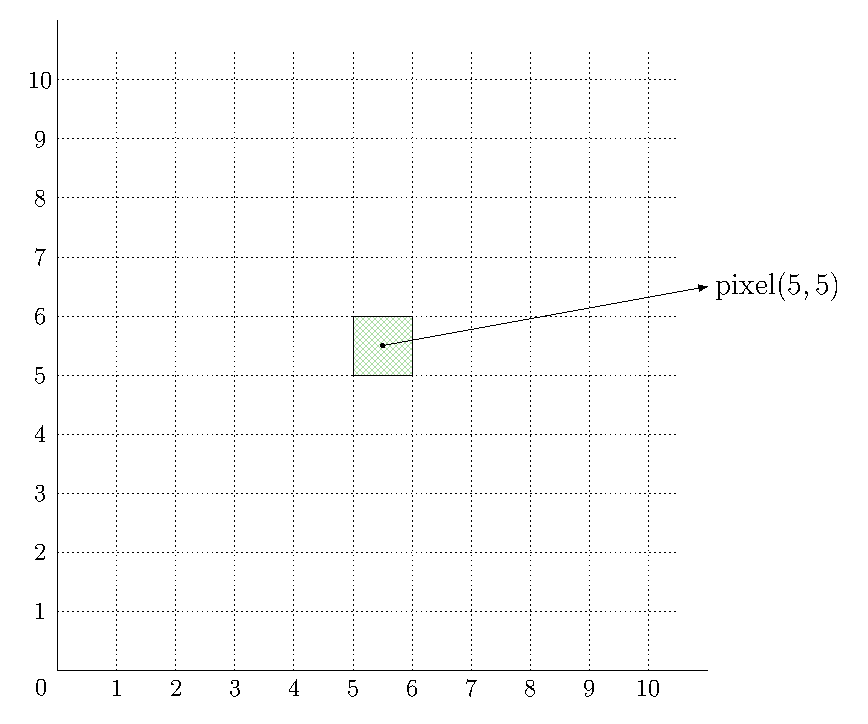
\includegraphics[scale=0.5]{History/pixel-grid.pdf}
  \end{center}
  \caption{Μια οθόνη ανάλυσης $10\times 10$ και ο προσδιορισμός ενός pixel σε αυτή}
\end{figure}

\begin{definition}
	Όταν αναφερόμαστε στη θέση ένος pixel με τις συντεταγμένες $(x,y)$ θα εννοούμε ότι το κέντρο του τετραγώνου βρίσκεται σε αυτή τη θέση πάνω στο πλέγμα, που συνθέτει την οθόνη μας.	
\end{definition}
%
\begin{remark}
	Το pixel για τα γραφικά είναι ότι είναι το σημείο για τα μαθηματικά. Αν και πρακτικά έχει διαστάσεις, σε αντίθεση με το σημείο, θεωρούμε ότι είναι ισοδύναμα.
\end{remark}
%
Με αυτόν τον τρόπο απεικόνισης, χρειαζόμαστε να σκεφτούμε τρόπους για να μπορέσουμε να σχεδιάσουμε ακόμα και απλά σχήματα, όπως ένα ευθύγραμμο τμήμα ή έναν κύκλο. Καθώς οι τρόποι που γνωρίζουμε από τα μαθηματικά δεν μπορούν να βρουν άμεση εφαρμογή.
Οι αλγόριθμοι αυτοί θα πρέπει να επιλέγουν το καλύτερο δυνατό pixel έτσι ώστε το τελικό αποτέλεσμα να είναι όσο πιο κοντά στο σχήμα που θέλουμε. Αλλά ταυτόχρονα ο υπολογισμός των pixel να γίνεται γρήγορα και χωρίς να χρειάζονται πολλές πράξεις ώστε να έχουμε σφάλματα λόγω της αριθμητικής του υπολογιστή και να χρησιμοποιούν ακεραίους.

\section{Σχεδιασμός ευθείας}

Για τον σχεδιασμό ευθυγράμμων τμημάτων υπάρχουν πολλοί αλγόριθμοι που θα μπορούσαμε να χρησιμοποιήσουμε, αλλά πρέπει να επιλέξουμε κάποιον που δεν θα παρουσιάζει προβλήματα κατά την υλοποίησή του.


\subsection{Αλγόριθμός Εξίσωσης Ευθείας}
Για παράδειγμα θα μπορούσαμε να χρησιμοποιήσουμε την αλγεβρική εξίσωση της ευ θείας για να προσδιορίσουμε ποια σημεία της ευθείας θα αντιστοιχούν σε pixel της οθόνης που θα επιλέξουμε να φωτίσουμε.

Αν θέλουμε να σχεδιάσουμε το ευθύγραμμο τμήμα $\olsi{P_1 P_2}$, με $P_1 = 
(x_1, y_1)$ και $P_2 = (x_2, y_2)$, τότε θα ισχύει:

\begin{equation*}
	\cfrac{y-y_1}{x-x_1} = \cfrac{y_2-y_1}{x_2-x_1} \Rightarrow y = \cfrac{y_2-y_1}{x_2-x_1}x + \cfrac{y_1x_2-y_2x_1}{x_2-x_1}
\end{equation*}
Θέτοντας, $S = \cfrac{y_2-y_1}{x_2-x_1}$ (κλίση) και $C = \cfrac{y_1x_2-y_2x_1}{x_2-x_1}$, προκύπτει ότι: $y=Sx+c$. Με βάση αυτή την εξίσωση, γράφουμ τον ακόλουθο αλγόριθμό:


\textbf{\underline{Βήμα 1:}} Διάβασε $P_1 = (x_1, y_1)$ και $P_2 = (x_2, y_2)$. \newline 
\textbf{\underline{Βήμα 2:}} Υπολόγισε $S = \cfrac{y_2-y_1}{x_2-x_1}$ (κλίση) και $C = \cfrac{y_1x_2-y_2x_1}{x_2-x_1}$. \newline 
\textbf{\underline{Βήμα 3:}} Για $x$ από $x_1$ έως $x_2$ με βήμα 1, υπολόγισε το $y = round(Sx+C)$ και φώτισε το pixel $(x,y)$. 
	
\begin{lstlisting}[caption={Plot Line Algorithm}]
function (x1, y1, x2, y2)
	if x1 == x2
		x = x1
		for y= y1:y2
			plot(x,y)
        end    
        return
	end	
    
    # Compute the slope
    s = (y2-y1)/(x2-x1)
    
    c = (y1x2-y2x1)/ (x2-x1)
    for x= x1:x2
    	y = round(sx +c)
    	plot(x,y)
    end    
end
\end{lstlisting}

Παρατηρούμε ότι ο αλγόριθμος έχει μικρή απαιτεί 1 flop για κάθε σημείο που θα εμφανιστεί στην οθόνη συντεταγμένη. Τα σημεία αυτά θα είναι όσα η διαφορά των τετμημένων των 2 σημείων μεταξύ των οποίων θέλουμε να σχηματίσουμε την ευθεία.

\begin{application}[Εφαρμογή του αλγορίθμου plot-line]
		Να εφαρμοστεί ο αλγόριθμος plot-line για τα ζεύγη σημείων:
\begin{enumerate}
	\item[$\mathrm{i)}$] $P_1 = (1, 1), P_2 = (3, 2)$
	\item[$\mathrm{ii)}$] $P_1 = (1, 1), P_2 = (4, 13)$
	\item[$\mathrm{iii)}$] $P_1 = (0, 0), P_2 = (0, 10)$	
\end{enumerate}

\begin{solution}
		

\begin{enumerate}
	\item[$\mathrm{i)}$] $P_1 = (1, 1), P_2 = (3, 2)$ \newline 
		\textbf{\underline{Βήμα 1}} (Υπολογισμός $s$):	
		\[
		s = \frac{y_2 - y_1}{x_2 - x_1} = \frac{2 - 1}{3 - 1} = \frac{1}{2} = 0.5
		\] 	
		
		\textbf{\underline{Βήμα 2}} (Υπολογισμός $c$):	
		\[
		c = \frac{y_1 x_2 - y_2 x_1}{x_2 - x_1} = \frac{1 \cdot 3 - 2 \cdot 1}{3 - 1} = \frac{3 - 2}{2} = \frac{1}{2} = 0.5	
		\]
		\textbf{\underline{Βήμα 3}} (Υπολογισμός και φωτισμός σημείων):		
		\begin{align*}
		   \text{For } x = 1: & \quad y = \text{round}(0.5 \cdot 1 + 0.5) = \text{round}(1) = 1 \\
		   \text{For } x = 2: & \quad y = \text{round}(0.5 \cdot 2 + 0.5) = \text{round}(1.5) = 2 \\
		   \text{For } x = 3: & \quad y = \text{round}(0.5 \cdot 3 + 0.5) = \text{round}(2) = 2 \\
		\end{align*}
		Άρα συνολικά θα φωτιστούν τα σημεία: \( (1, 1), (2, 2), (3, 2) \).
		
		\begin{figure}[hbt]
		  \begin{center}
			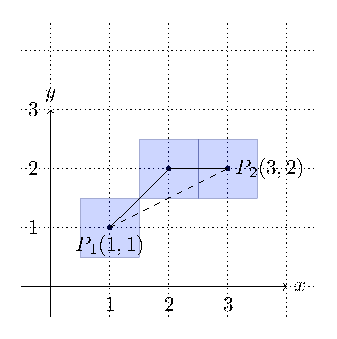
\includegraphics[scale=1]{Chapter1/Plot-Line/application1a.pdf}
		  \end{center}
		  \caption{Φωτισμένα σημεία έπειτα από εφαρμογή αλγορίθμου Plot Line για τα σημεία $P_1 = (1,1), P_2 = (3,2)$}
		\end{figure}


	\item[$\mathrm{ii)}$] $P_1 = (1, 1), P_2 = (4, 13)$ \newline 
		\textbf{\underline{Βήμα 1}} (Υπολογισμός $s$):
		\[
		   s = \frac{13 - 1}{4 - 1} = \frac{12}{3} = 4
		\]
		
		\textbf{\underline{Βήμα 2}} (Υπολογισμός $c$):
		   \[
		   c = \frac{1 \cdot 4 - 13 \cdot 1}{4 - 1} = \frac{4 - 13}{3} = \frac{-9}{3} = -3
		   \]
		
		\textbf{\underline{Βήμα 3}} (Υπολογισμός και φωτισμός σημείων):	
		   \begin{align*}
		   \text{For } x = 1: & \quad y = \text{round}(4 \cdot 1 - 3) = \text{round}(1) = 1 \\
		   \text{For } x = 2: & \quad y = \text{round}(4 \cdot 2 - 3) = \text{round}(5) = 5 \\
		   \text{For } x = 3: & \quad y = \text{round}(4 \cdot 3 - 3) = \text{round}(9) = 9 \\
		   \text{For } x = 4: & \quad y = \text{round}(4 \cdot 4 - 3) = \text{round}(13) = 13 \\
		   \end{align*}
		Άρα συνολικά θα φωτιστούν τα σημεία: \( (1, 1), (2, 5), (3, 9), (4, 13) \).	
	
	\item[$\mathrm{iii)}$]  \( P_1 = (0, 0), P_2 = (0, 10) \) \newline 
		Εφόσον τα σημεία $P_1, P_2$ έχουν την ίδια τετμημένη, τότε θα σχεδιάσουμε την κάθετη γραμμή που τα ενώνει. 	
		Άρα συνολικά θα φωτιστούν τα σημεία: $ (0, 0), (0, 1), (0, 2), \ldots, (0, 10) $.
		
		\begin{figure}[h!]
			\begin{minipage}[b]{0.48\textwidth} % Top-left image	
				\begin{center}
				    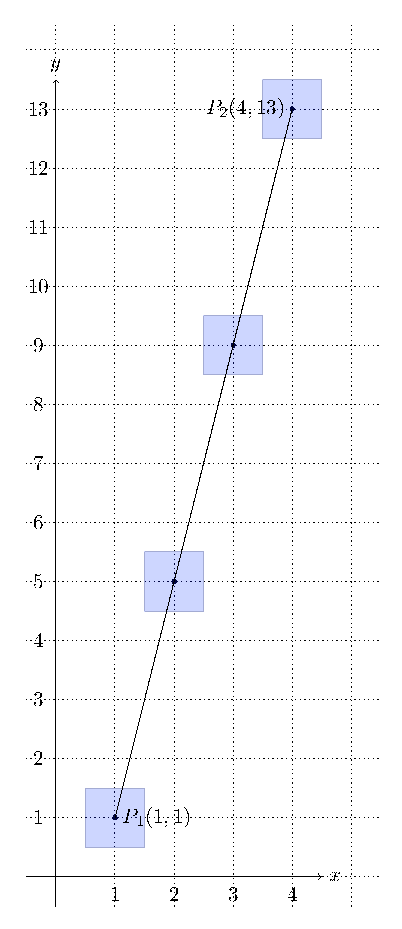
\includegraphics[scale=0.7]{Chapter1/Plot-Line/application1b.pdf}
				\end{center}    
			\end{minipage}%
			\hfill
			\begin{minipage}[b]{0.48\textwidth} % Top-right image
			    \begin{center}
				    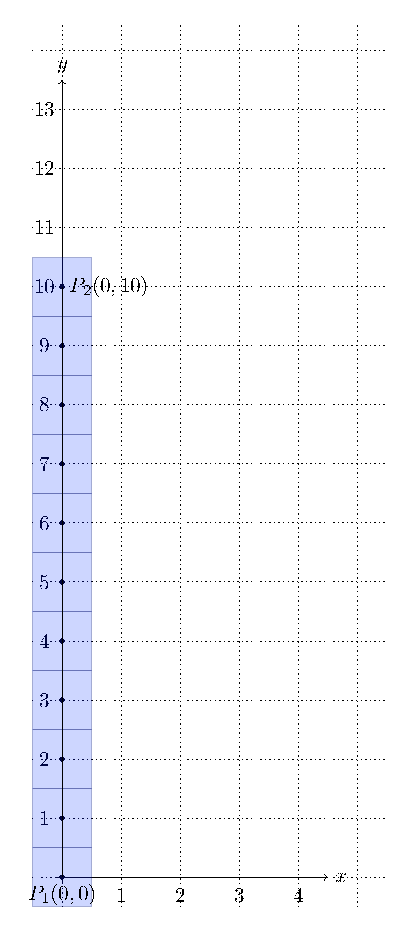
\includegraphics[scale=0.7]{Chapter1/Plot-Line/application1c.pdf}
				\end{center}    
			\end{minipage}
			\caption{Φωτισμένα σημεία έπειτα από εφαρμογή αλγορίθμου Plot Line για τα σημεία $P_1 = (1,1), P_2 = (3,2)$}
		\end{figure}

\end{enumerate}


\end{solution}
	
\end{application}

\subsection{Μειονεκτήματα Αλγορίθμου εξίσωσης ευθείας}

Αν χρησιμοποιήσουμε αυτόν τον αλγόριθμο θα παρατηρήσουμε ότι για ζεύγη σημείων το ευθύγραμμο τμήμα μας θα παρουσιάζει κενά και δεν θα είναι συνεχές.

Συγκρεκριμένα, αν η κλίση είναι μεγαλύτερη του $1$, τότε ο αλγόριθμος δε φωτίζει συνεχόμενα pixel.
Αυτό το πρόβλημα, μπορεί να διορθωθεί, εκφράζοντας το $x$ σα συνάρτηση του $y$.

\[
	x = f(y) = \cfrac{x_2 - x_1}{y_2- y_1}y +  \cfrac{ y_2 x_1 - y_1 x_2  }{ y_2 - y_1 } 
\]

 Επίσης κατά τον υπολογισμό των τιμών πραγματοποιούμε πολλαπλασιασμούς και διαιρέσεις που αυξάνουν την πολυπλοκότητα και εισάγουν και αριθμητικά σφάλματα στα δεδομένα μας. Κάθε σημείο απαιτεί για τον υπολογισμό του \texttt{1 flop + 1 rounding}, άρα η πολυπλοκότητα του αλγορίθμου είναι αυξημένη.
 
 Για αυτούς τους λόγους η χρήση της αλγεβρικής εξίσωσης της ευθείας σε υπολογιστή δεν είναι βέλτιστη. Ευτυχώς έχουν ήδη αναπτυχθεί άλλοι τρόποι που θα μας βοηθήσουν να υπολογίσουμε ποια πιξελ θα πρέπει να φωτίσουμε στην οθόνη για να σχηματιστεί το ζητούμενο ευθύγραμμο τμήμα. Ένα τέτοιος είναι ο αλγόριθμος ευθυγράμμων τμημάτων του Bresenham.






\subsection{Αλγόριθμος Bresenham για ευθύγραμμο τμήμα}

Το $1965$ ο J.E. Bresenham παρουσίασε την πρώτη DDA μέθοδο (Digital Differential Analyzer) για το σχεδιασμό ευθύγραμμου τμήματος. Εκεί παρουσίαζε τη μορφή που έχει ο αλγόριθμός του για ευθύγραμμα τμήματα που ανήκουν στο πρώτο οκταμόριο. Δηλαδή που η γωνία που σχηματίζουν με τον οριζόντιο άξονα είναι από $0$ εώς $\ang{45}$. Καθώς και τις μετατροπές που χρειάζονται να γίνουν για να μπορούμε να σχεδιάσουμε ευθύγραμμα τμήματα κάθε κλίσης.


\begin{figure}[h!]
  \begin{center}
	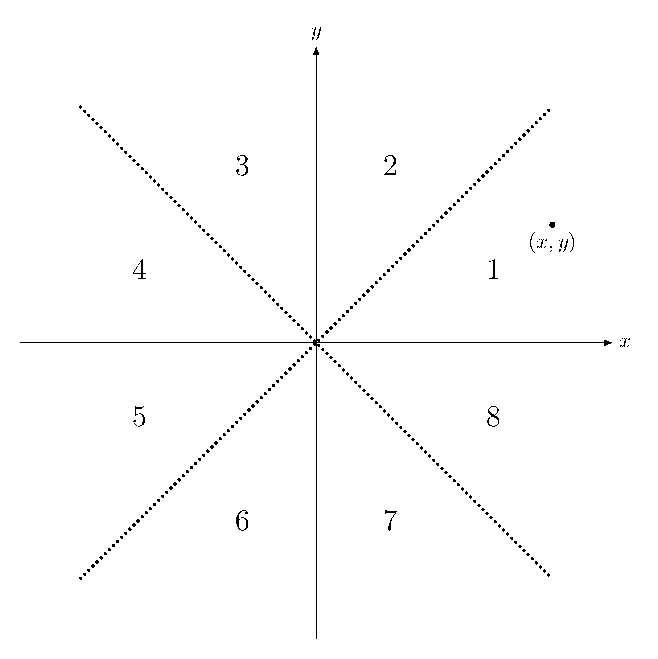
\includegraphics[scale=0.5]{Chapter1/Bresenham/octamoriums.pdf}
  \end{center}
  \caption{Τα οκταμόρια του επιπέδου}
\end{figure}


Προσδιορίζουμε το σχεδιασμό της ευθείας στο $1$ο οκταμόριο και στη συνέχεια με κατάλληλη τροποποίηση, που θα την περιγράψουμε παρακάτω, μπορούμε να επεκταθούμε και στα άλλα οκταμόρια.

΄Εστω ότι θέλουμε να σχεδιάσουμε ένα ευθύγραμμο τμήμα $\overline{P_1 P_2}$, για pixels τα οποία ανήκουν στο $1$ο οκταμόριο, έστω $P_1= (x_1, y_1), P_2= (x_2, y_2)$. 

Έστω ότι έχει φωτισθεί στην οθόνη το pixel $P_i (x_i , y_i)$.

\begin{figure}[h!]
  \begin{center}
	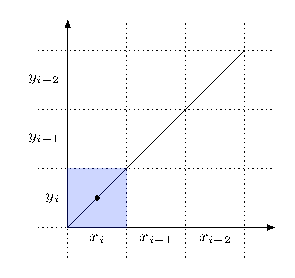
\includegraphics{Chapter1/Bresenham/bresenham-stepwise/bresenham-zero.pdf}
  \end{center}
  \caption{Σχεδιασμός ευθύγραμμου τμήματος μεταξύ των pixel στο $1$ο οκταμόριο}
\end{figure}





Δεδομένου ότι ο σχεδιασμός του ευθυγράμμου τμήματος συνίσταται στον επιλεκτικό φωτισμό διαδοχικών pixels ώστε αυτά να σχηματίζουν ευθύγραμμο τμήμα, θεωρούμε ότι αφού βρισκόμαστε στο 1ο οκταμόριο εάν ήδη είναι φωτισμένο το pixel $P_i(x_i , y_i)$ τα επόμενα δυνατά προς φωτισμό pixels θα είναι τα $P_{i+1}(x_{i+1} , y_i)$ ή $P_{i+1}(x_{i+1} , y_{i+1})$

Παρατηρούμε δηλαδή ότι οπωσδήποτε θα αυξηθεί κατά $1$ η συντεταγμένη x και η συντεταγμένη y ή θα παραμείνει ίδια ή θα αυξηθεί κι αυτή κατά $1$. Θα πρέπει, λοιπόν να καθορίσουμε μία μεταβλητή σφάλματος, η οποία ανάλογα να αποφαίνεται εάν θα αυξηθεί ή όχι η συντεταγμένη $y$.

\subsection{Δημιουργία μεταβλητής σφάλματος $\epsilon_i$}

Η εξίσωση μεταξύ των σημείων $(x_i,y_i)$ και $(x_{i + 1}, y)$ είναι  
%
\[
	y =sx_{i+1}+c, 
\]
όπου,
\begin{align*}
	s &= \cfrac{y-y_i}{x_i+1-x_i} = \cfrac{\Delta y}{\Delta x} \leq 1, \text{η κλίση της ευθέιας} \\
	c &= \cfrac{y_i x_{i+1} - y x_i}{x_{i+1}-x_i}
\end{align*}
%
%
Υπολογίζουμε τις αποστάσεις $d_1, d_2$ και της διαφορά τους $d_1-d_2$:

\begin{align*} 
	d_1 &= y-y_i = s(x_i+1)+c-y_i \\
	d_2 &= (y_i+1)-y = y_i+1- s(x_i+1)-c \\
	d_1-d_2 &= 2s(x_i+1) - 2y_i +2c-1
\end{align*}

\begin{figure}[hbt]
  \begin{center}
	  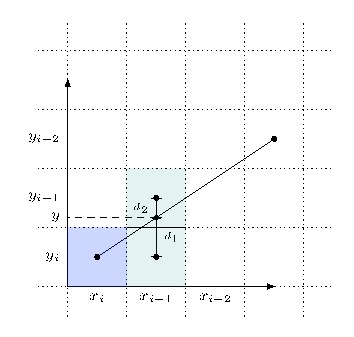
\includegraphics[]{Chapter1/Bresenham/bresenham-stepwise/bresenham-first-step.pdf}
  \end{center}
  \caption{}
\end{figure}



\begin{remark}
	 Ανάλογα με το πρόσημο της διαφοράς $d_1-d_2$ μπορούμε να επιλέξουμε το επόμενο προς φωτισμό pixel. 	
\end{remark}

Εάν ονομάσουμε μεταβλητή σφάλματος, $e_i$, την ποσότητα $e_i = \Delta x(d_1 − d_2)$ τότε θα έχουμε :

\begin{table}[h!]
\centering
\begin{tabular}{cc}
\toprule
$e_i$      & Επόμενο προς φωτισμό pixel \\
\midrule
$< 0$      & $(x_i+1, y_i)$ \\
$\geq 0$   & $(x_i+1, y_i+1)$ \\
\bottomrule
\end{tabular}
\caption{Πίνακας με κριτήριο προσδορισμού επόμενο προς φωτισμό pixel.}
\label{tab:next_pixel}
\end{table}


\subsection{Προσπάθεια δημιουργίας αναδρομικού τύπου}

Σε κάθε βήμα σχεδιασμού της ευθείας θα είναι καλό να μπορούμε να υπολογίζουμε την καινούρια μεταβλητή σφάλματος συναρτήσει της προηγούμνηες, γι' αυτό προσπαθούμε να δημιουργήσουμε έναν αναγωγικό τύπο. Ισχύει ότι:

\begin{equation*}
	e_i = \Delta x(d_1-d_2).	
\end{equation*}

%
Καθώς,
%
\begin{equation*}
	  \left.\begin{aligned}
	  s &= \cfrac{\Delta y}{\Delta x}	\\
	  d_1 &= y-y_i = s(x_i+1)+c-y_i\\
	  d_2 &= (y_i+1)-y = y_i+1- s(x_i+1)-c	
	\end{aligned}\right\} \Rightarrow e_i = \cfrac{\Delta y}{s} (2s(x_i+1)-2y_i+2c-1)
\end{equation*}
 Αφού όμως, $\cfrac{\Delta y}{s} = \Delta x$, συνολικά έχουμε ότι:
 %
\begin{align*}
	e_i = 2\Delta y(x_i+1) - 2\Delta xy_i + \Delta x(2c − 1) 
		= 2\Delta yx_i - 2\Delta xy_i +c', \quad c' = 2\Delta y + \Delta x(2c − 1) \tag{1}
 	\label{eq:1}
\end{align*}
%
Λόγω της \eqref{eq:1}, για το $e_{i+1}$ θα ισχύει: 
%
\begin{equation*}
	e_{i+1} = 2\Delta yx_{i+1} − 2\Delta xy_{i+1} + c'.
\end{equation*}
%
Τελικά,
%
\begin{align*}
	e_{i+1}-e_i &= 2\Delta yx_{i+1} − 2\Delta xy_{i+1} + c'- 2\Delta yx_i + 2\Delta xy_i -c' = \\\
				&= 2\Delta y (x_{i+1}-x_i)-2\Delta x(y_{i+1}-y_i)		
\end{align*}
%
Για $i=1$, $(x_1,y_1) \equiv (0,0)$. Οπότε, αξιοποιώντας την \eqref{eq:1}, λαμβάνουμε:

\begin{itemize}
	\item $c = \cfrac{y_i x_{i+1} - y x_i}{x_{i+1}-x_i} 
  =	\cfrac{y_1 \cdot(x_1+1) - y \cdot x_1}{x_1+1-x_1}
  = 0 \cdot(0+1) - y \cdot 0
  = 0 $
	\item $e_1 = 2\Delta y \cdot 0 - 2\Delta x\cdot 0 +2\Delta y + \Delta x (2c-1) 
	= 2\Delta y + 2\Delta x \cdot c - \Delta x \overset{c=0}{=} 2\Delta y - \Delta x$
\end{itemize}
%
Προκύπτει, λοιπόν, ότι:
%
\begin{table}[h!]
\centering
\begin{tabular}{l c}
\toprule
\multicolumn{1}{c}{$e_1$} & \multicolumn{1}{c}{Επόμενη μεταβλητή σφάλματος $e_2$} \\
\midrule
$< 0 \to (x_i+1, y_i)$       & $e_1 + 2\Delta y$                  \\
$\geq 0 \to (x_i+1, y_i+1)$  & $e_1 + 2\Delta y - 2\Delta x$      \\
\bottomrule
\end{tabular}
\caption{Πίνακας με τις συνθήκες και τις μεταβλητές σφάλματος.}
\label{tab:error_conditions}
\end{table}


\begin{figure}[h!]
\begin{center}
\begin{minipage}[b]{0.48\textwidth} % Top-left image
%    \centering
    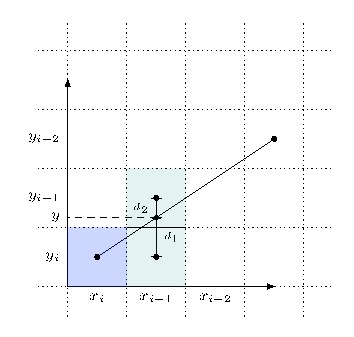
\includegraphics[width=\textwidth]{Chapter1/Bresenham/bresenham-stepwise/bresenham-first-step.pdf}
    \captionof{figure}{Top-Left Image}
\end{minipage}%
\hfill
\begin{minipage}[b]{0.48\textwidth} % Top-right image
%    \centering
    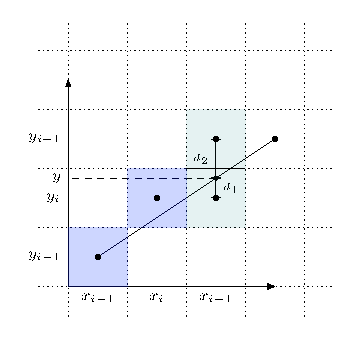
\includegraphics[width=\textwidth]{Chapter1/Bresenham/bresenham-stepwise/bresenham-second-step.pdf}
    \captionof{figure}{Top-Right Image}
\end{minipage}

\vspace{1em} % Add vertical space

\noindent
\begin{minipage}[b]{0.48\textwidth} % Bottom-left image
%    \centering
    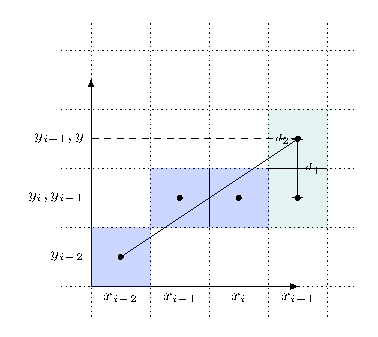
\includegraphics[width=\textwidth]{Chapter1/Bresenham/bresenham-stepwise/bresenham-third-step.pdf}
    \captionof{figure}{Bottom-Left Image}
\end{minipage}%
\hfill
\begin{minipage}[b]{0.48\textwidth} % Bottom-right image
%    \centering
    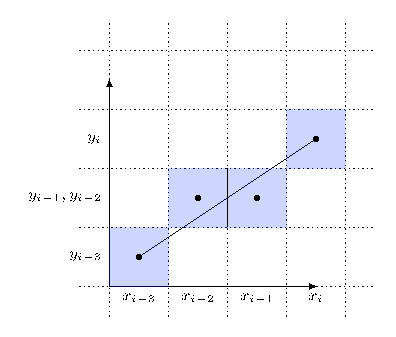
\includegraphics[width=\textwidth]{Chapter1/Bresenham/bresenham-stepwise/bresenham-fourth-step.pdf}
    \captionof{figure}{Bottom-Right Image}
\end{minipage}
\end{center}
\end{figure}

\subsection{Υλοποίηση αλγορίθμου για 1ο Οκταμόριο}

\subsubsection{Συνάρτηση ``φωτισμού" pixel}

Η παρακάτω συνάρτηση, παίρνει σαν είσοδο τις συντεταγμένες ενός σημείου στο επίπεδο, $\mathbb{R}^2$ και εκτυπώνει γράφημα με χρωματισμένο τετράγωνο πλευράς $1$ και κέντρο, το σημείο με τις συντεταγμένες της εισόδου:

\begin{lstlisting}[caption={Julia function to draw a rectangle}]
function draw_rectangle(x, y, color, test=true)
    # Define the coordinates of the rectangle vertices
    x_vertices = [x - 0.5, x + 0.5, x + 0.5, x - 0.5, x - 0.5]
    y_vertices = [y - 0.5, y - 0.5, y + 0.5, y + 0.5, y - 0.5]
    
    # Plot the rectangle
    if test    
        plot(x_vertices, y_vertices, aspect_ratio=:equal, 
             color=color, fill=true, legend=false, alpha=0.5)
        scatter!([x], [y], color=:red, aspect_ratio=:equal)
    else     
        plot!(x_vertices, y_vertices, aspect_ratio=:equal, 
              textwidth=2, color=color, fill=true, legend=false, alpha=0.7)
    end    
end
\end{lstlisting}

Οπότε, αν ο χρήστης εισάγει τις συνταταγμένες 2 σήμειων, έστω $P_1(x_1,y_1), P_2(x_2,y_2)$, τα οποία ανήκουν στο $1$ο οκταμόριο, τότε καλώντας παραπάνω αλγόριθμο, λαμβάνουμε τα κέντρα των pixel που σχεδιάζουν την ευθεία Bresenham που ενώνει τα $2$ σημεία.

\begin{example}
\end{example}


\begin{lstlisting}[caption={Bresenham Line Algorithm for 1st Octant}]
	function Bresenham_first_oct(x1, y1, x2, y2) 
	    dx = x2 - x1
	    dy = y2 - y1
	    x = x1
	    y = y1
	    c1 = 2 * dy
	    e = 2 * dy - dx
	    c2 = e - dx
	    
	    # Initialize L matrix with data points (x2-x1+1 points)
	    L = zeros(Int, 2, dx + 1)
	    
	    L[1, 1] = x #x coordinates in 1st row
	    L[2, 1] = y #2 coordinates in 2nd row
	
	    while x <= x2
	        L[1, x - x1 + 1] = x
	        L[2, x - x1 + 1] = y
	        
	        x += 1
	        if e < 0
	            e += c1
	        else
	            y += 1
	            e += c2
	        end
	    end
	    return [L[1,:], L[2,:]]
	end
\end{lstlisting}

\subsection{Σκιαγράφηση μεθόδου για σημεία εκτός 1ου οκταμορίου}

Αρκεί να εξετάσουμε τη συμπεριφορά της μεθόδου για τα οκταμόρια $1, 2, 3, 4$ (γιατί;)
 
Στην αρχική ιδέα του Bresenham παίζει σημαντικό ρόλο η σειρά που θα δώσουμε τα σημεία $P_1$ και $P_2$, Δηλαδή ποιο είναι η αρχή και ποιο το τέλος του τμήματος. Έτσι προκύπτουν 8 διαφορετικές περιπτώσεις. Αν, όμως, απλά θέλουμε να σχεδιάσουμε ένα ευθύγραμμο τμήμα, δεν μας ενδιαφέρει από ποια μεριά θα ξεκινήσουμε τον σχεδιασμό του. Συμφωνούμε να επιλέγουμε πάντα σαν αρχή το σημείο για την τετμημένη του οποίου ισχύει $y = min(y_1,y_2)$. Τότε, αντί για 8 περιπτώσεις, έχουμε μόνο 4, αφού τα οκταμόρια $5, 6, 7, 8$ ανάγονται σε $1, 2, 3, 4$ αντίστοιχα.

\begin{example}[Αναγωγή από 8ο οκταμόριο σε 4ο οκταμόριο]
	Έστω τα σημεία $P_1(2,-1), P_2(4,-3)$, τα οποία όπως είναι φανερό, ανήκουν στο $8$ο οκταμόριο.
\end{example}
%
%
\begin{figure}[h!]
  \begin{center}
	  \includegraphics[scale=1]{Chapter1/Bresenham/axis-transformation/figure1.pdf}
  \end{center}
  \caption{Πρώτο βήμα αναγωγής 8ου τεταρτημορίου σε 4ο}
\end{figure}
%
%
\textbf{Βήμα 1:} Διαλέγω σαν αρχή το στοιχείο που έχει μικρότερη τεταγμένη, δηλαδή το $P_2$, και μετονομάζω: $P_1 \to P_2'\quad \text{και} \quad P_2 \to P_1'$.
%
%

\begin{minipage}{\textwidth}
	\begin{minipage}[b]{0.5\textwidth} % Top-left image
	    \centering
	    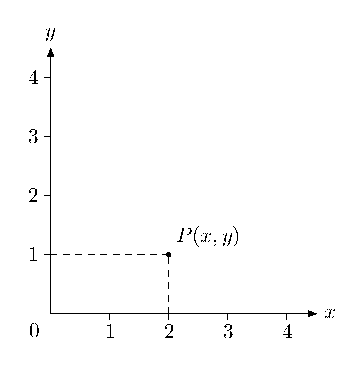
\includegraphics[width=\textwidth]{Chapter1/Bresenham/axis-transformation/figure2a.pdf}
%	    \captionof{figure}{Top-Left Image}
	\end{minipage}%
	\hfill
	\begin{minipage}[b]{0.5\textwidth} % Top-right image
	    \centering
	    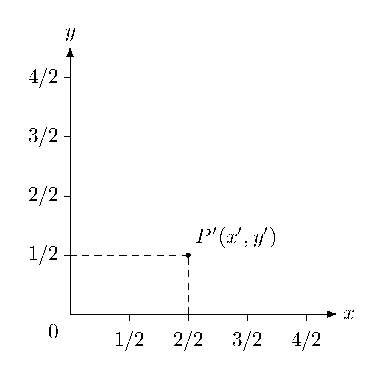
\includegraphics[width=\textwidth]{Chapter1/Bresenham/axis-transformation/figure2b.pdf}
	\end{minipage}
	\captionof{figure}{Επιλέγοντας αρχή των νέων αξόνων το σημείο με τη μικρότερη συντεταγμένη}
\end{minipage}
%
%
\textbf{Βήμα 2:} Παρατηρώ, φέρνοντας νέους νοητούς ορθοκανονικούς άξονες με αρχή το $P_1'$, ότι το ευθύγραμμό τμήμα που καλούμαι να σχεδιάσω σύμφωνα με τον αλγόριθμο του Bresenham ανήκει στο 4o Οκταμόριο.


\begin{minipage}{1\textwidth}
	\begin{minipage}[b]{0.48\textwidth} % Top-left image
	    \centering
	    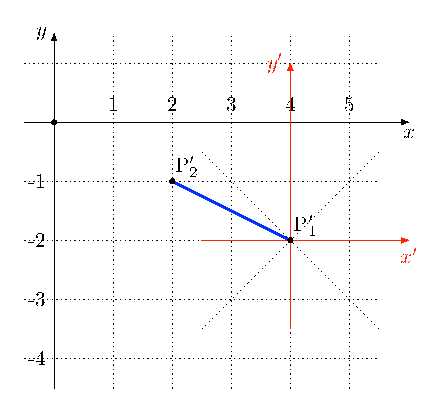
\includegraphics[width=\textwidth]{Chapter1/Bresenham/axis-transformation/figure3a.pdf}
%	    \captionof{figure}{Top-Left Image}
	\end{minipage}%
	\hfill
	\begin{minipage}[b]{0.48\textwidth} % Top-right image
	    \centering
	    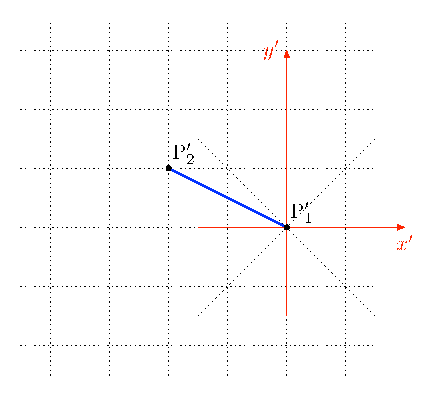
\includegraphics[width=\textwidth]{Chapter1/Bresenham/axis-transformation/figure3b.pdf}
	\end{minipage}
	\captionof{figure}{Επιλέγοντας αρχή των νέων αξόνων το σημείο με τη μικρότερη συντεταγμένη}
\end{minipage}

%% 2o oktamorio
\subsection{Αλγόριθμος του Bresenham για σημεία στο 2ο οκταμόριο}

Έστω $P_1(x_1,y_1), P_2(x_2,y_2)$, τα οποία ανήκουν στο $2$ο οκταμόριο. Ο σχεδιασμός της ευθείας του Bresenham στο $2$ο οκταμόριο γίνεται αν χρησιμοποιήσουμε στον αλγόριθμο του Bresenham τα συμμετρικά τους ως προς την $1$η διχοτόμο, δηλαδή τα σημεία $P_1' = (y_1, x_1)$ και $P_2' = (y_2, x_2)$. Τότε, εκμεταλλευόμενοι τη συμμετρία αυτή, αντί να φωτίζουμε το pixel $(x, y)$ που θα μας επιστρέφει ο αλγόριθμος εμείς φωτίζουμε το $(y, x)$. 

\begin{remark}
	Ο φωτισμός των συμμετρικών ως προν την 1η διχοτόμο pixel που θα προκύψουν από τον αλγόριθμο του Bresenham μπορεί να γίνει μία και καλή όταν περατωθεί ο αλγόριθμος. Αυτό μπορεί να συμβεί καθώς ο αλγόριθμος που έχουμε διατυπώσει επιστρέφει τα σημεία που πρέπει να φωτιστούν για να σχηματιστεί η επιθυμητή ευθεία. 
\end{remark}

\begin{minipage}{1\textwidth}
	\begin{minipage}[b]{0.48\textwidth} % Top-left image
	    \centering
	    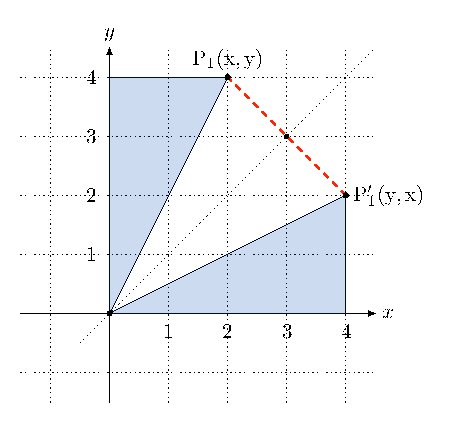
\includegraphics[width=\textwidth]{Chapter1/Bresenham/symmetries/symmetry-2nd.pdf}
%	    \captionof{figure}{Top-Left Image}
	\end{minipage}%
	\hfill
	\begin{minipage}[b]{0.48\textwidth} % Top-right image
	    \centering
	    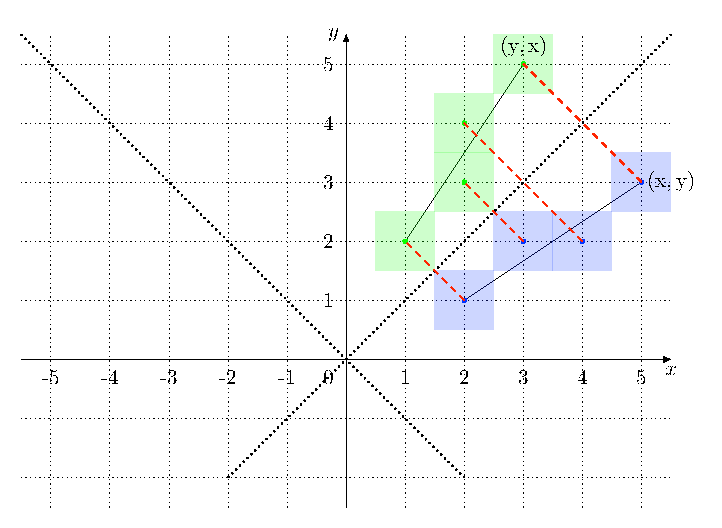
\includegraphics[width=\textwidth]{Chapter1/Bresenham/symmetries/bresenham-2nd.pdf}
	\end{minipage}
	\captionof{figure}{Συμμετρία μεταξύ 1ου και 2ου οκταμορίου που εκμεταλλεύομαστε για σηματισμό ευθείας σύμφωνα με αλγόριθμο του bresenham}
\end{minipage}

\begin{lstlisting}[caption={Bresenham Line Algorithm for 2nd Octant}]
function Bresenham_second_oct(x1, y1, x2, y2) 
	xPoints1, yPoints1 = Bresenham_first_oct(y1, x1, y2, x2)  
    for i in 1:xPoints1[end] - xPoints1[1]+1
        draw_rectangle(xPoints1[i], yPoints1[i], "blue", false)
		draw_rectangle(yPoints1[i], xPoints1[i], "green", false)
    end
endfunction    
\end{lstlisting}


%% 3o oktamorio
\subsection{Αλγόριθμος του Bresenham για σημεία στο 3ο οκταμόριο}

Έστω $P_1(x_1,y_1), P_2(x_2,y_2)$, τα οποία ανήκουν στο $3$ο οκταμόριο. Ο υπολογισμός των σημείων στο $3$ο οκταμόριο γίνεται αν θεωρήσουμε ότι στη θέση των $P_1$ και $P_2$, εισάγουμε τα σημεία $P_1' = (y_1, -x_1)$ και $P_2' = (y_2, -x_2)$. Τότε, αντί να φωτίζουμε το pixel $(x, y)$ που θα μας επιστρέφει ο αλγόριθμος εμείς φωτίζουμε το $(y, -x)$. Αυτό βέβαια, δεν είναι αναγκαίο να το κάνουμε σε κάθε βήμα του αλγορίθμου· μπορούμε να το κάνουμε μία και καλή, όταν περατωθεί ο αλγόριθμος.


\begin{minipage}{1\textwidth}
	\begin{minipage}[b]{0.48\textwidth} % Top-left image
	    \centering
	    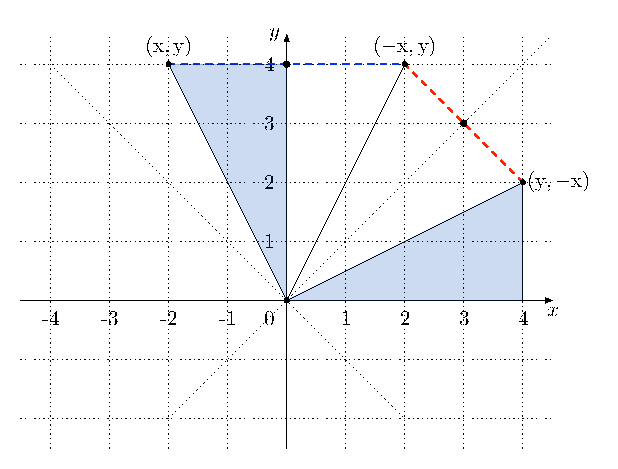
\includegraphics[width=\textwidth]{Chapter1/Bresenham/symmetries/symmetry-3rd.pdf}
%	    \captionof{figure}{Top-Left Image}
	\end{minipage}%
	\hfill
	\begin{minipage}[b]{0.48\textwidth} % Top-right image
	    \centering
	    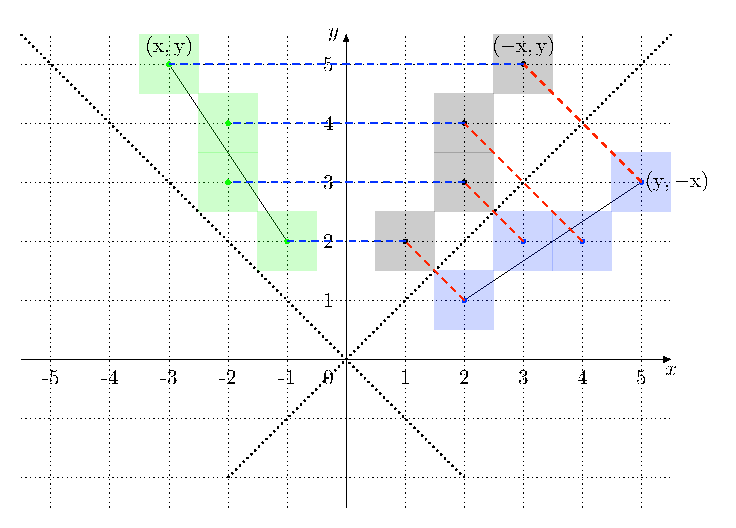
\includegraphics[width=\textwidth]{Chapter1/Bresenham/symmetries/bresenham-3rd.pdf}
	\end{minipage}
	\captionof{figure}{Συμμετρία μεταξύ 1ου και 2ου οκταμορίου που εκμεταλλεύομαστε για σηματισμό ευθείας σύμφωνα με αλγόριθμο του bresenham}
\end{minipage}

\begin{lstlisting}[caption={Bresenham Line Algorithm for 3rd Octant}]
function Bresenham_second_oct(x1, y1, x2, y2) 
	#(y1, -x1) and (y2, -x2) are the symmetric of (x1, y1) and (x2, y2) respectively in the 1st octant
	
	xPoints1, yPoints1 = Bresenham_first_oct(y1, -x1, y2, -x2)  
    for i in 1:xPoints1[end] - xPoints1[1]+1
        draw_rectangle(xPoints1[i], yPoints1[i], "blue", false)
		draw_rectangle(yPoints1[i], xPoints1[i], "gray", false)        
		draw_rectangle(-yPoints1[i], xPoints1[i], "green", false)
    end
endfunction    
\end{lstlisting}



%% 4o oktamorio
\subsection{Αλγόριθμος του Bresenham για σημεία στο 4ο οκταμόριο}

Έστω $P_1(x_1,y_1), P_2(x_2,y_2)$, τα οποία ανήκουν στο $4$ο οκταμόριο. Ο υπολογισμός των σημείων στο $4$ο οκταμόριο γίνεται αν θεωρήσουμε ότι στη θέση των $P_1$ και $P_2$, εισάγουμε τα σημεία $P_1' = (-x_1, y_1)$ και $P_2' = (-x_2, y_2)$ και αντί για να φωτίζουμε το pixel $(x, y)$ που θα μας επιστρέφει ο αλγόριθμος εμείς φωτίζουμε το $(-x, y)$. Αυτό βέβαια, δεν είναι αναγκαίο να το κάνουμε σε κάθε βήμα του αλγορίθμου· μπορούμε να το κάνουμε μία και καλή, όταν περατωθεί ο αλγόριθμος.


\begin{minipage}{1\textwidth}
	\begin{minipage}[b]{0.48\textwidth} % Top-left image
	    \centering
	    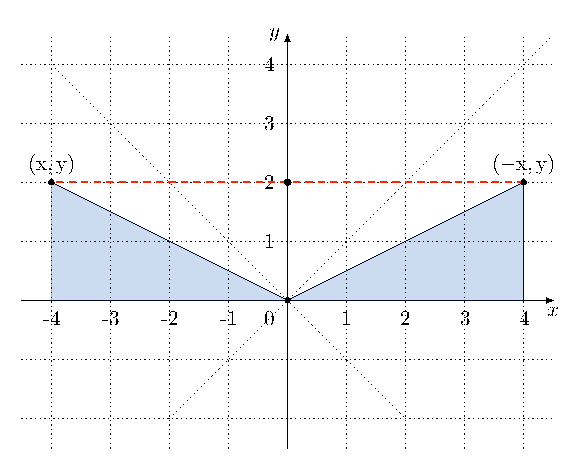
\includegraphics[width=\textwidth]{Chapter1/Bresenham/symmetries/symmetry-4th.pdf}
%	    \captionof{figure}{Top-Left Image}
	\end{minipage}%
	\hfill
	\begin{minipage}[b]{0.48\textwidth} % Top-right image
	    \centering
	    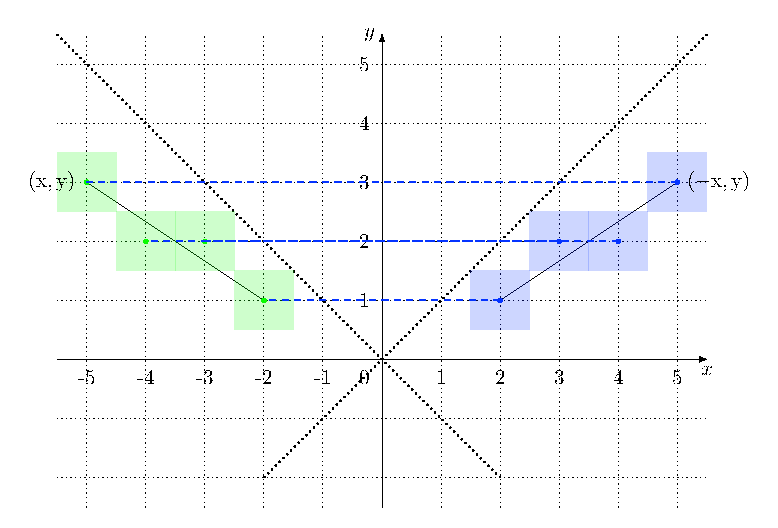
\includegraphics[width=\textwidth]{Chapter1/Bresenham/symmetries/bresenham-4th.pdf}
	\end{minipage}
	\captionof{figure}{Συμμετρία μεταξύ 1ου και 2ου οκταμορίου που εκμεταλλεύομαστε για σηματισμό ευθείας σύμφωνα με αλγόριθμο του Bresenham}
\end{minipage}

\begin{lstlisting}[caption={Bresenham Line Algorithm for 4th Octant}]
function Bresenham_second_oct(x1, y1, x2, y2) 
	#(-x1, y1) and (-x2, y2) are the symmetric of (x1, y1) and (x2, y2) respectively in the 1st octant
	
	xPoints1, yPoints1 = Bresenham_first_oct(-x1, y1, -x2, y2)  
    for i in 1:xPoints1[end] - xPoints1[1]+1
        draw_rectangle(xPoints1[i], yPoints1[i], "blue", false)
		draw_rectangle(-xPoints1[i], yPoints1[i], "green", false)        
    end
endfunction    
\end{lstlisting}

\subsection{Γενικός Αλγόριθμος Bresenham}
	Αν συνδυάσουμε όλα τα παραπάνω τότε προκύπτει ο παρακάτω αλγόριθμος που σχεδιάζει ευθεία που ενώνει δύο σημεία που παρίστανται στο επίπεδο σύμφωνα με τη λογική του αλγορίθμου του Bresenham.
	
	
\begin{lstlisting}[caption={General Bresenham Line Algorithm}]
function Bresenham_line(x1, y1, x2, y2)
	# Select starting point with the smallest y coordinate
    if y2 < y1
        x1, x2 = x2, x1
        y1, y2 = y2, y1
    end       
	# Find octants
    dx = x2 - x1
    dy = y2 - y1
    s = dy/dx
    if s <= 1 && s >= 0 # oct 1
        xPoints, yPoints = Bresenham_first_oct(x1, y1, x2, y2)  
    elseif s > 1 # oct 2
        xPoints, yPoints = Bresenham_first_oct(y1, x1, y2, x2) 
        
        xPoints, yPoints = yPoints, xPoints #from 1st octant, back to 2nd so i switch xPoints with yPoints

    elseif s < -1 # oct 3
        xPoints, yPoints = Bresenham_first_oct(y1, -x1, y2, -x2) 
        #from 1st octant, back to 3rd: 
            xPoints, yPoints = yPoints, xPoints #1. switch xPoints with yPoints to go to 2nd octant 
            
            xPoints, yPoints = -xPoints, yPoints #2. mirror with respect to new xPoints to go from 2nd to third

    else # oct 4
        xPoints, yPoints = Bresenham_first_oct(-x1, y1, -x2, y2)
        
        xPoints, yPoints = -xPoints, yPoints #from 1st octant, back to 4rd so: mirror with respect to xPoints 
    end
    
    # return [xPoints,yPoints]

    scatter(xPoints, yPoints, markersize=3, xlabel="x", ylabel="y", legend=false)
    # plot(xPoints, yPoints, xlabel="x", ylabel="y", legend=false, lc=:red) uncomment to add line

    for i in 1:size(xPoints,1)
        draw_rectangle(xPoints[i], yPoints[i], "blue", false)
    end

    plot!(title = "Bresenham line: ($x1,$y1) -> ($x2,$y2)", aspect_ratio=1)
    scatter!(xPoints, yPoints, markersize=3, xlabel="x", ylabel="y", legend=false)
    #savefig("giannis/outputs/line.png")   
endfunction
\end{lstlisting}	
	
\section{Σχεδιασμός του Κύκλου}
\subsection{Σχεδιασμός Κύκλου μέσω της αλγεβρικής εξίσωσης}

Έστω κύκλος με κέντρο $K(x_c, y_c)$ και ακτίνα $r$. Τότε η αλγεβρική του εξίσωση είναι:
\begin{equation}
	(x-x_c)^2 + (y-y_c)^2 = r^2
	\label{eq:1}
\end{equation}

Λύνωντας την $\eqref{eq:1}$ ως προς $y$ προκύπτει:
\[
	y = f(x) = y_c \pm \sqrt{r^2- (x-x_c)^2}
\]

Είναι προφανές, ότι απαιτούνται πολλοί υπολογισμοί σε κάθε βήμα. Σαν να μην έφτανε αυτό, απαιτείται και υπολογισμός της τετραγωνικής ρίζας, που "βαραίνει" ακόμα περισσότερο τους υπολογισμούς μας.

Αυτό έχει ως αποτέλεσμα, να μην είναι ομοιόμορφη η κατανομή των φωτιζόμενων pixelσ και ειδικά στο κομμμάτι μεταξύ $45^\circ$ και $90^\circ$.

\begin{lstlisting}[caption={Αλγόριθμος Σχεδιασμού κύκλου μέσω αλγεβρικής εξίσωσης}]
function circlePlot(xc, yc, r)
	# (xc, yc) are the coordinates of the circle's centre
	# r is the radius of the circle
	x = xc-r 
    i = 1
	while x <= xc+r
        y1 = yc + sqrt( r^2-(x-xc)^2 )
        plot(x,y1)
        y2 = yc - sqrt( r^2-(x-xc)^2 )
        plot(x,y2)
        x = x + 1 
	end
end
\end{lstlisting}


\begin{figure}[hbt]
  \begin{center}
	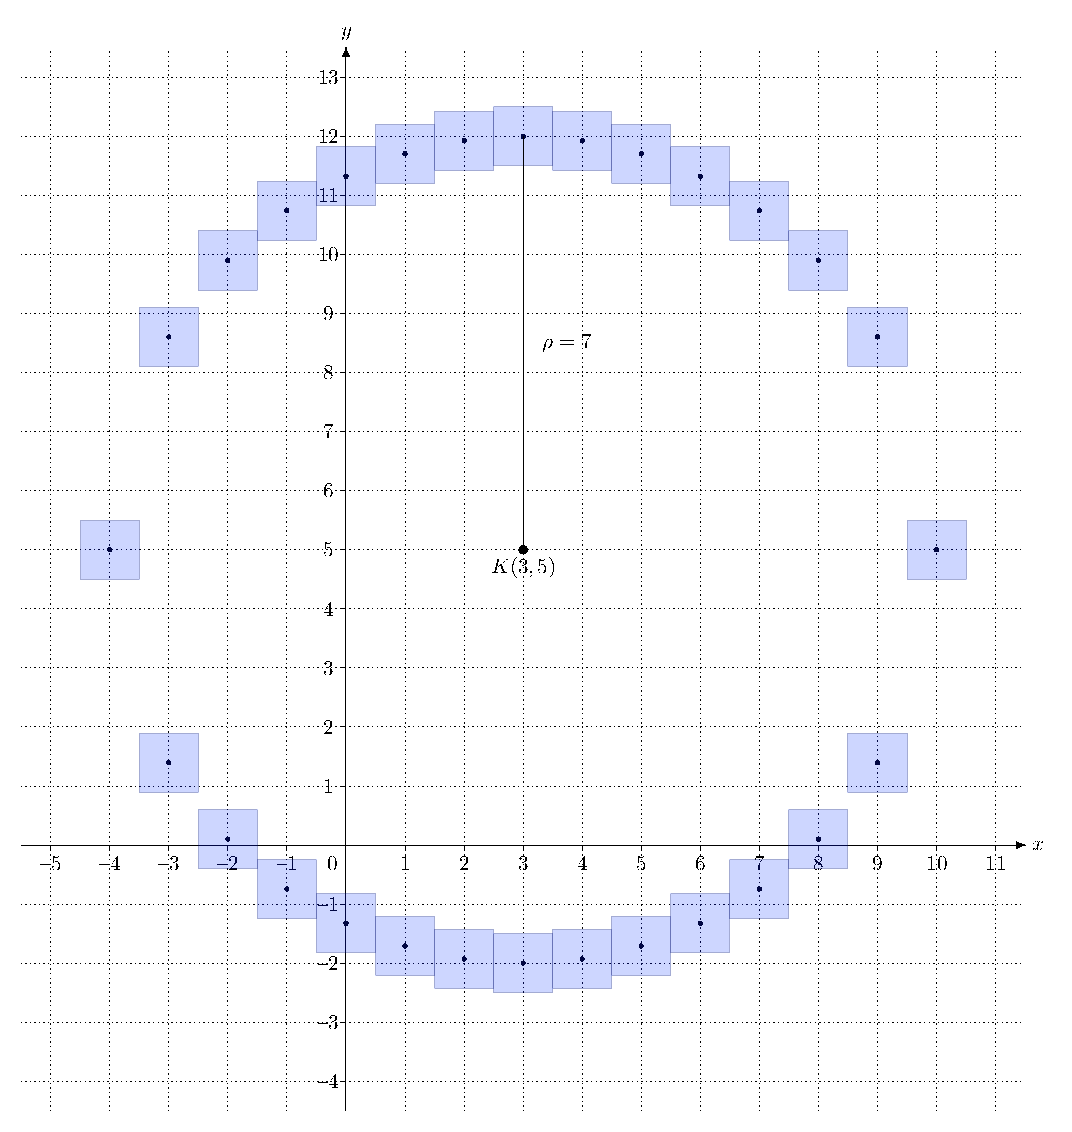
\includegraphics[scale=0.6]{Chapter1/Circle/plot-circle.pdf}
  \end{center}
  \caption{Σχεδιασμός κύκλου κέντρου $K(3,5)$ και ακτίνας $r=7$ μέσω αλγεβρικής εξίσωσης}
\end{figure}

Ο αλγόριθμος αυτός μπορεί να βελτιωθεί αν χρησιμοποιήσουμε τις παραμετρικές εξισώσεις για τις συντεταγμένες του κύκλου.
\begin{equation*}
	  \left.\begin{aligned}
	  x(t) &= x_c + r\cos{t}\\
	  y(t) &= y_c + r\sin{t}
	\end{aligned}\right. \, , \, t \in [0, 2\pi]
\end{equation*}

\begin{lstlisting}[caption={Αλγόριθμος Σχεδιασμού Κύκλου μέσω παραμετρικής εξίσωσης}]
function circlePlot(xc, yc, r, iterations)
    # xc, yc are the coordinates of the circle's center
    # r is the radius of the circle

    theta_values = range(0, 2π, length=iterations)  # Even partition of [0, 2π]

    x_points = Float64[]  # To store x(t)
    y_points = Float64[]  # To store y(t)

    for t in theta_values
        x = xc + r * cos(t)
        y = yc + r * sin(t)
        push!(x_points, x)
        push!(y_points, y)
    end

    return x_points, y_points  # Return arrays of x and y coordinates
end
\end{lstlisting}



\begin{figure}[h!]
  \begin{center}
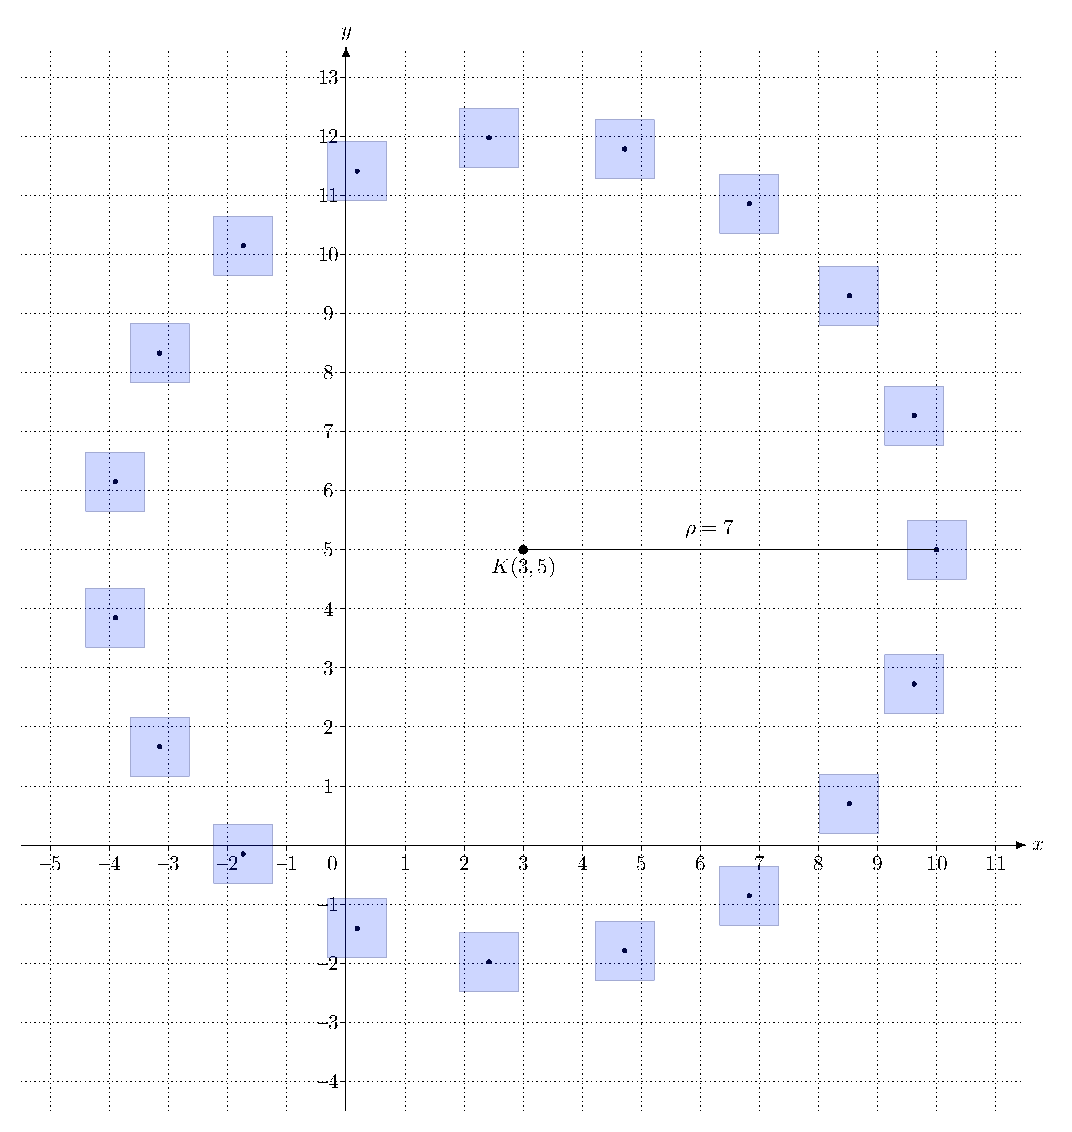
\includegraphics[scale=0.6]{Chapter1/Circle/circle-parametric.pdf}
  \end{center}
  \caption{Σχεδιασμός κύκλου κέντρου $K(3,5)$ και ακτίνας $r=7$ μέσω παραμετρικών εξισώσεων}
\end{figure}

Ενώ ο τρόπος αυτός σχεδιασμός κύκλου έχει πολύ καλά αποτελέσματα όσο αυξάνεται ο αριθμός επαναλήψεων (\texttt{iterations}), είναι αρκετά απαιτητικός καθώς απαιτεί για κάθε επανάληψη τις τιμές τριγωνομετρικών συναρτήσεων.
%%%%%%%%%%%%%%%%%%%%%%%%%%%%%%%%%%%%%%%%%%

\subsection{Σχεδιασμός κύκλου με τον Αλγόριθμο του Bresenham}

Ο κύκλος είναι ένα συμμετρικό σχήμα. Κάθε αλγόριθμος για τη σχεδίαση ενός κύκλου μπορεί να εκμεταλλευτεί αυτή τη συμμετρία για να σχεδιάσει $8$ σημεία υπολογίζοντας μόνο ένα. Αυτό αποτελεί τη λεγόμενη συμμετρία των $8$ δρόμων.

\begin{figure}[h!]
  \begin{center}
  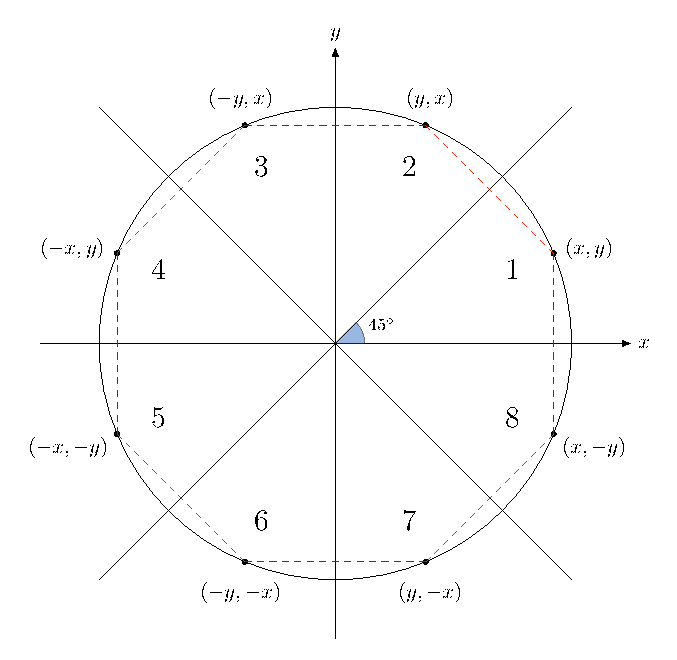
\includegraphics[scale=0.7]{Chapter1/Circle/8-street.pdf}
  \end{center}
  \caption{Συμμετρία των 8 δρόμων}
\end{figure}


Έστω ότι θέλουμε να σχεδιάσουμε το $2$ο οκτομόριο ενός κύκλου κέντρου $(0,0)$ και ακτίνας $\rho$. Εάν υπολογίσουμε όλα τα σημεία αυτού του οκταμορίου τα υπόλοιπα μπορούν να προσδιοριστούν χρησιμοποιώντας τη συμμετρία των $8$ δρόμων.


\subsection{Καθορισμός της μεταβλητής απόφασης}


Εάν φωτιστεί το pixel $(x_i, y_i)$ στο $2$ο οκταμόριο. Τα επόμενα δυνατά προς φωτισμό pixel θα είναι τα $(x_i + 1, y_i)$ ή $(x_i + 1, y_i - 1)$. 

\begin{figure}[hbt]
  \begin{center}
	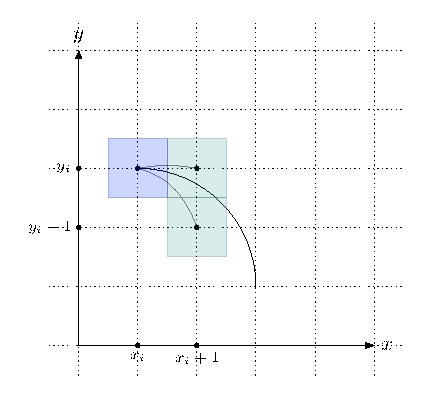
\includegraphics[scale=1]{Chapter1/Circle/circle-next-step.pdf}
  \end{center}
  \caption{Δίλημμα επιλογής επόμενου προς χρωματισμό pixel κατά τον σχεδιασμό του κύκλου σύμφωνα με τον αλγόριθμο του Bresenham}
\end{figure}

Θα πρέπει να καθορίσουμε μια μεταβλητή απόφασης ανάλογα με την οποία να επιλέγουμε εάν η συντεταγμένη $y$ θα παραμείνει ίδια ή θα ελαττωθεί, δεδομένου ότι η συντεταγμένη $x$ σταθερά θα αυξάνεται κατά $1$. 

Έστω ότι συντεταγμένη $x_{i+1}$ αντιστοιχεί σε κάποιο $y$ ανάμεσα στις τιμές $y_i$ και $y_i-1$. Είναι γνωστό ότι το σημείο $(x_i +1, y)$ θα ανήκει στον κύκλο, επομένως  το $y$ ικανοποιεί τη σχέση:
\[
	y^2 = r^2 - x_{i+1}^2.
\]

Ορίζουμε τις ακόλουθες διαφορές $d_1$ και $d_2$
\begin{align*}
	d_1 &= y_i^2 - y^2 = y_i^2 - r^2 + x_{i+1}^2 \\
	d_2 &= y^2 - \color{red}{(y_i-1)^2} = r^2 - x_{i+1}^2 - (y_i - 1)^2
\end{align*}

Εάν θέσουμε $e_i = d_1 - d_2$ τότε αυτή αποτελεί μεταβλητή απόφασης ανάλογα με το πρόσημο της οποίας μπορούμε να επιλέξουμε το επόμενο προς φωτισμό σημείο. Παρατηρούμε ότι


\begin{table}[htb]
\centering
	\begin{tabular}{@{}c|c@{}}
    \toprule
    $e_i$   & Επόμενο προς φωτισμό pixel \\ \midrule
    $<0$    & $(x_i + 1, y_i)$           \\
    $\geq 0$ & $(x_i + 1, y_i - 1)$      \\ \bottomrule
    \end{tabular}
\end{table}

Ο Bresenham απέδειξε ότι μία ικανοποιητική μεταβλητή απόφασης για την επιλογή του κατάλληλου pixel στο βήμα $i$ είναι η $e_i = d_1 - d_2$.


\subsection{Δημιουργία αναδρομικού τύπου}

Η μεταβλητή απόφασης $e_i$ μπορεί να υπολογισθεί ως εξής: 

\begin{align*}
	e_i &= d_1 - d_2 = 
		  y_i^2 - r^2 + (x_i +1)^2 - r^2 + (x_i +1)^2 + (y_i-1)^2 =  \\ 
		&=  2(x_i +1)^2 + y_i^2 + (y_i -1)^2 -2r^2	
\end{align*}
%
Επομένως:
%
\begin{align*}
	e_{i+1} &= 2(x_{i+1} + 1)^2 + y_{i+1}^2 + (y_{i+1}-1)^2 - 2r^2 = \\
			 &= 2(x_i +2)^2 + y_{i+1}^2 + (y_{i+1} -1)^2 - 2r^2 = \\
			 &= 2x_i^2 + 8x_i + 8 + y_{i+1}^2 + y_{i+1}^2 -2y_{i+1} + 1 -2r^2 = \\
			 &= (2x_i^2 + 4x_i +2) + 4x_i + 6 + 2y_{i+1}^2 -2y_{i+1} +1-r^2 = \\
			 &= 2(x_i +1)^2 + 4x_i + 6 + 2y_{i+1}^2 - 2y_{i+1} + 1 -2r^2 = \\
			 &= e_i - y_i^2 - y_i^2 + 2y_i -1 + 4x_i + 6 + 2y_{i+1}^2 -2y_{i+1} + 1 = \\
			 &=  e_i + 4x_i + 6 + 2(y_{i+1}^2 - y_i^2) -2(y_{i+1} - y_i)
\end{align*}
%
Άρα:
%
\begin{equation}
	e_{i+1} = e_i + 4x_i + 6 + 2(y_{i+1}^2 - y_i^2) -2(y_{i+1}-y_i)
	\label{eq:2}
\end{equation}


Επειδή στη σχεδίαση του $2$ου οκταμορίου ξεκινάμε από το $(x_1, y_1) = (0,r)$, η αρχική μεταβλητή απόφασης $e_1$ είναι:
%
\begin{align*}
	e_1 = 2+r^2 + (r-1)^2 - 2r^2 = 
		2+r^2 + r^2 -2r+1-2r^2 = 
		3-2r.
\end{align*}

Επειδή στο δεύτερο οκταμόριο η τιμή του $y_{i+1}$ είναι $y_i$ ή $y_i -1$ (μεγαλύτερη ταχύτητα στη $x$ κατεύθυνση) μπορούμε να υπολογίσουμε το $e_{i+1}$ με βάση το πρόσημο του $e_i$ ως εξής.

\begin{itemize}
  \item $e_i < 0 \Rightarrow y_{i+1} = y_i$. Τότε η \eqref{eq:2} γίνεται:
  \[
	   e_{i+1} = e_i + 4(x_i +1) + 2 \Rightarrow e_{i+1} = e_i + 4(x_i + 1) + 2
   \]
   \item $e_i \geq 0 \Rightarrow y_{i+1} = y_i - 1$. Τότε η \eqref{eq:2} γίνεται:
   \begin{align*}
   	e_{i+1} &= e_i + 4x_i  + 6 + 2( (y_i -1)^2 - y_i^2 ) - 2(y_i -1 -y_i) =  \\
   			&= e_i + 4x_i + 6 + 2(y_i^2 -2y_i + 1 -y_i^2) + 2 = \\ 
 			&= e_i + 4(x_i + 1) + 2 -4(y_i -1)
   \end{align*}
   
\end{itemize}

Ανάλογα λοιπόν με το πρόσημο της μεταβλητής $e_i$ έχουμε:

\begin{table}[htb]
\centering
    \begin{tabular}{@{}c|c@{}}
        \toprule
        $e_i$    & $e_{i+1}$                         \\ \midrule
        $<0$     & $e_i + 4(x_i +1) +2$              \\
        $\geq 0$ & $e_i + 4(x_i +1) +2 - 4(y_i - 1)$ \\ \bottomrule
    \end{tabular}
\end{table}



\subsection{Αλγόριθμος Bresenham για κύκλο}

Για να σχεδιάσουμε κάποιο κύκλο με διαφορετικό κέντρο, αρκεί να παρατηρήσουμε αν εφαρμόσουμε μετασχηματισμό μεταφοράς, ότι ένα σημείο της περιφέρειας ενός τέτοιου κύκλου μπορεί να σχεδιαστεί αν μεταφέρουμε τον κύκλο με κέντρο το $(0,0)$ κατά διάνυσμα με συντεταγμένες το κέντρο του κύκλου. Έτσι προκύπτει ο ακόλουθος αλγόριθμος υλοποιημένος σε Julia.

Τα παραπάνω μας οδηγούν στον παρακάτω αλγόριθμο χρησιμοποιώντας και την συμμετρία των $8$ δρόμων.

\begin{lstlisting}[caption={Bresenham Circle Algorithm}]
function bresenhamCircle(r)
	# (xc, yc) are the coordinates of the circle's centre
	# r is the radius of the circle
	x = 0 
	y = r
	error = 3 - 2 * r
	
	while x <= y
		plot(x, y)
		 
		plot(x+xc, y+yc, 0)
		plot(x+xc, -y+yc, 0) 
		plot(-x+xc, y+yc, 0) 
		plot(-x+xc, -y+yc, 0) 
		plot(y+xc, x+yc, 0) 
		plot(-y+xc, x+yc, 0)
		plot(y+xc, -x+yc, 0) 
		plot(-y+xc, -x+yc, 0) 
		x = x + 1
		if error > 0
			y = y - 1
			error = error - 4*y
		end
		error = error + 4*x +2
	end
end
\end{lstlisting}



\begin{figure}[hbt]
  \begin{center}
	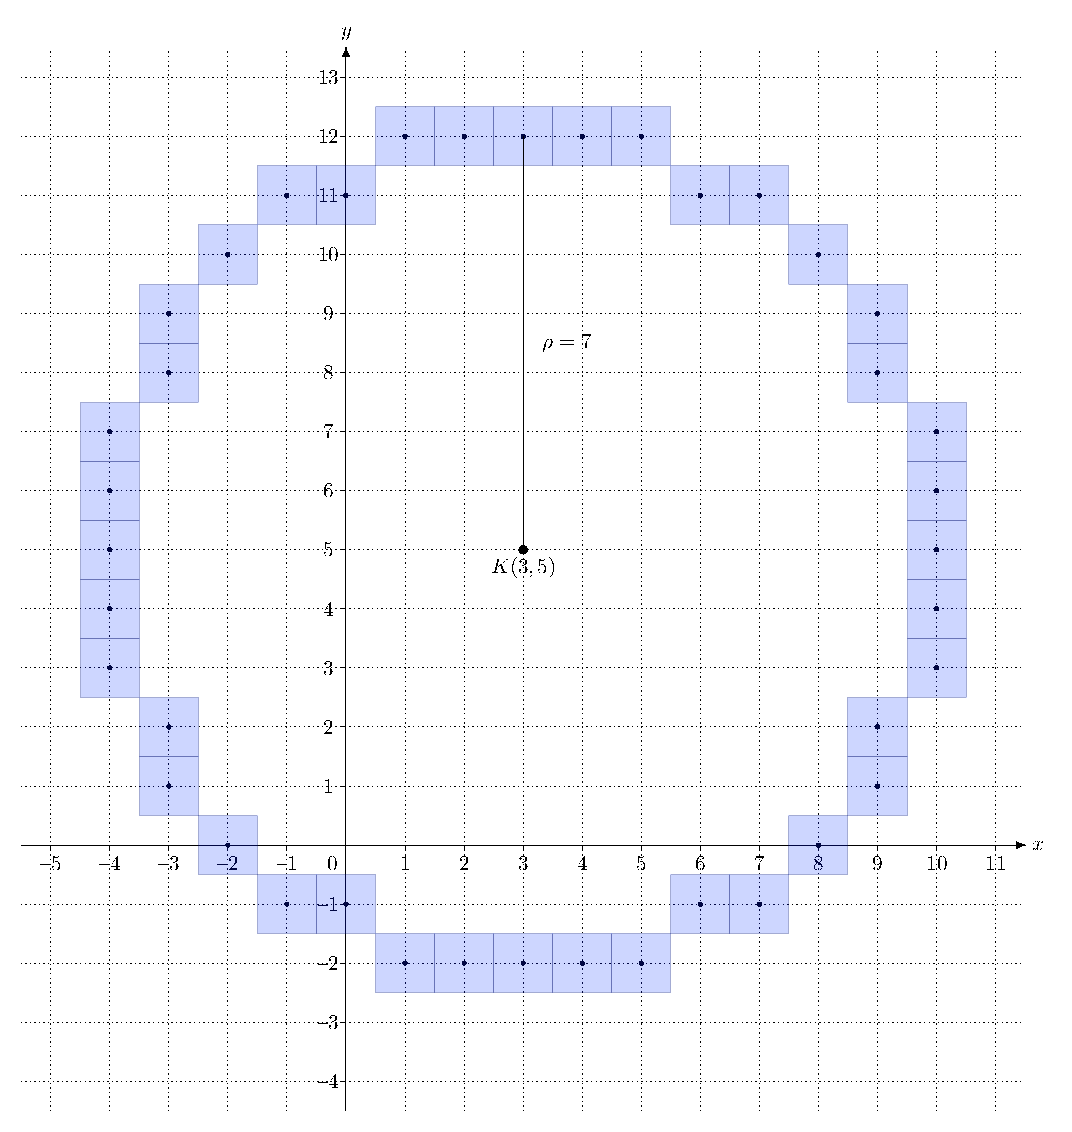
\includegraphics[scale=0.6]{Chapter1/Circle/bresenham-circle-example.pdf}
  \end{center}
  \caption{Παράδειγμα κύκλου με κέντρο $K(3,5)$ και ακτίνα $\rho = 7$}
\end{figure}


\subsection{Υπολογιστική Πολυπλοκότητα}

Στο $2$ο οκταμόριο ισχύει : $0 \leq r\cos{\ang{45}}, r \sin{\ang{45}} \leq  y \leq  r$. Στην $x$ κατεύθυνση γίνονται $r \cos{\ang{45}}$ βήματα που αντιστοιχούν σε $ r(1 - \sin{\ang{45}})$ βήματα στην $y$ κατεύθυνση. Συνολικά σχεδιάζονται (υπολογίζονται) $r \cos{\ang{45}}$ σημεία.


\begin{figure}[hbt]
  \begin{center}
	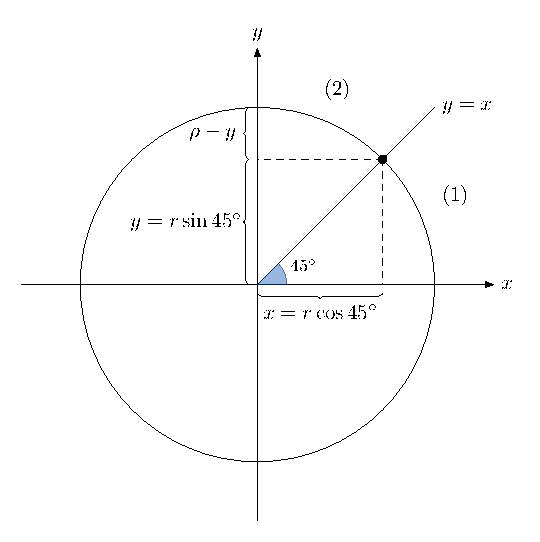
\includegraphics[scale=1]{Chapter1/Circle/circle-complexity.pdf}
  \end{center}
  \caption{Παράδειγμα κύκλου με κέντρο $K(3,5)$ και ακτίνα $\rho = 7$}
\end{figure}





Μέσος όρος βημάτων:
\[
	\left( \cfrac{r\cfrac{\sqrt{2}}{2} + r - r\cfrac{\sqrt{2}}{2} }{r\cfrac{\sqrt{2}}{2}} \right) = \sqrt{2}
\]


Η εντολή \texttt{error = error + 4x + 2} περιλαμβάνει $2$ προσθέσεις, $1$ shift πράξη (πολλαπλασιασμός με $2$). Τελικά κατά μέσο όρο έχουμε $4\sqrt{2}$ προσθέσεις, $2$ shift και $\sqrt{2}$ increments (αυξήσεις) ανά σχεδίαση σημείου του κύκλου.
Αν οι πράξεις εντός του \texttt{while} απαιτούν $1$ κύκλο hardware, τότε για το $2$ο οκταμόριο απαιτούνται $\sqrt{2}$ κύκλοι ανά σημείο. Για ολόκληρο κύκλο $(7+ 2) /8$ κύκλοι ανά σημείο, δηλαδή $1.05$ κύκλοι ανά σημείο.
\begin{remark}
Τα συνολικά σημεία που σχεδιάζονται στον κύκλο είναι $8r \cos{\ang{45}} = 4r \sqrt{2}$. Συγκρινόμενα με την περίμετρο $2 \pi\rho$ είναι $10\%$ λιγότερα. 
\end{remark}

\section{Σχεδιασμός Έλλειψης}

    Έστω ότι θέλουμε να σχεδιάσουμε έλλειψη με κέντρο το $O (0,0)$ και άξονες με διάμετρο $2a$ και $2b$, $a, b \in \mathbb{Z}$. Η έλλειψη χαρακτηρίζεται από 4πλή συμμετρία.

\begin{figure}[hbt]
  \begin{center}
	\includegraphics[scale=1]{Figures/Chapter1/Ellipse/figure1.pdf}
  \end{center}
  \caption{Έλλειψη}
\end{figure}

Ο διαχωρισμός σε περιοχή 1 και περιοχή 2 γίνεται εκεί όπου

\[
\frac{dy}{dx} = -1
\]
Εξίσωση Έλλειψης

\[
\frac{x^2}{a^2} + \frac{y^2}{b^2} = 1
\]

\[
f(x,y) = b^2x^2 + a^2y^2 - a^2b^2 = 0
\]
\subsection{Υπολογιστική Πολυπλοκότητα}

\begin{tabular}{m{0.2\textwidth}m{0.4\textwidth}}
	  Περιοχή 1: & \( y_r \) βήματα της \( y \)-κατεύθυνσης.\\
	& \( a - x_r \) βήματα της \( x \)-κατεύθυνσης.\\
	& Υπολογίζονται \( y_r \) σημεία.
\end{tabular}

\begin{tabular}{m{0.2\textwidth}m{0.4\textwidth}}
	Περιοχή 2: & \( x_r \) βήματα της \( x \)-κατεύθυνσης.\\
	& \( b - y_r \) βήματα της \( y \)-κατεύθυνσης.\\
	& Υπολογίζονται \( x_r \) σημεία.
\end{tabular}

Για \( (1) \) βήμα στην \( y \)-κατεύθυνση στην περιοχή 1 απαιτούνται 3 προσθέσεις (ανάλογα για τα βήματα της \( x \)-κατεύθυνσης της περιοχής 2) ανά σημείο κατά μέσο όρο:
\[
\frac{3y_r + 2(a-x_r) +3x_r + 2(b-y_r)}{ x_r +y_r} = 1+ 2\frac{a+b}{\sqrt{a^2 + b^2 }}, \text{ προσθέσεις, } \frac{a+b}{\sqrt{a^2 + b^2}} \text{ αυξήσεις ανά σημείο.}
\]

\begin{figure}[hbt]
  \begin{center}
	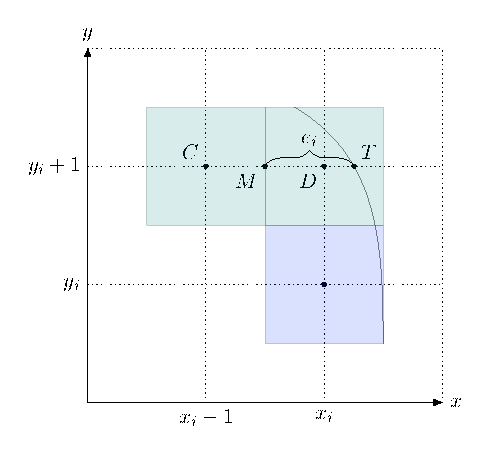
\includegraphics[scale=1]{Figures/Chapter1/Ellipse/figure2.pdf}
  \end{center}
  \caption{Περιοχή 1}
\end{figure}

\subsection*{Περιοχή 1:}
Έστω ότι έχει φωτισθεί το pixel $(x_i, y_i)$. Επειδή βρισκόμαστε στην περιοχή 1, το επόμενο προς φωτισμό pixel θα είναι το $(x_i, y_i+1)$ ή το $(x_i-1, y_i+1)$. Παρατηρούμε ότι αυξάνεται κατά 1 η $y$ συντεταγμένη και χρειαζόμαστε ένα κριτήριο.

Απόφαση για το αν θα φωτιστεί η $x_i$ ή $x_{i-1}$ θέση. Έστω $M$ το μέσο του ευθύγραμμου τμήματος $CD$. Οι συντεταγμένες του μέσου $M$ θα είναι

\begin{equation}
    f(M) = f \left( \frac{x_i + x_{i-1}}{2}, y_i + 1 \right) = f \left( x_i - \frac{1}{2}, y_i + 1 \right)
\end{equation}

Εάν $T$ είναι το σημείο τομής της έλλειψης με το ευθύγραμμο τμήμα $CD$ και $e_i$ η απόσταση από το μέσο $M$, τότε αυτό ικανοποιεί την εξίσωση της έλλειψης και θα ισχύει:

\begin{equation}
    f \left( x_i - \frac{1}{2} + e_1, y_i + 1 \right) = b^2 \left( x_i - \frac{1}{2} + e_1 \right)^2 + a^2 (y_i + 1)^2 - 4a^2b^2 = 0
\end{equation}

Αναπτύσσοντας την προηγούμενη έκφραση έχουμε ότι:

\begin{equation}
    f \left( x_i - \frac{1}{2}, y_i + 1 \right) = - \left( 2b^2 \left( x_i - \frac{1}{2} \right) e_1 + b^2 e_1^2 \right) = 0
\end{equation}

Εάν ονομάσουμε μεταβλητή απόφασης για την περιοχή 1, $f_{mid1}$ τις συντεταγμένες του μέσου $M$ θα έχουμε:

\begin{equation}
    f_{mid1} = f(M) = - \left( 2b^2 \left( x_i - \frac{1}{2} \right) e_1 + b^2 e_1^2 \right)
\end{equation}

Παρατηρούμε ότι το πρόσημο της έκφρασης του $f(M)$ καθορίζει την επιλογή του επόμενου σημείου. Συγκεκριμένα:

\begin{table}[htb]
    \centering
    \begin{tabular}{@{}c|c@{}}
        \toprule
        $f(M)$ & Επιλογή σημείου \\  \midrule
        $< 0$ & $e_1 > 0 \Rightarrow$ Το $T$ δεξιότερα του $M$, επιλογή του σημείου $D$ \\
        $\geq 0$ & $e_1 \leq 0 \Rightarrow$ Το $T$ αριστερότερα του $M$, επιλογή του σημείου $C$ \\
        \bottomrule
    \end{tabular}
\end{table}

\subsection{Αναδρομικός υπολογισμός των $f_{mid1}$ και $f_{mid2}$}

Είναι απαραίτητο να υπάρχει μια σχέση σύνδεσης ανάμεσα στις δύο μεταβλητές απόφασης. Έχουμε ότι Περιοχή 1:

\begin{equation}
    f_{mid1, i+1} = f(x_{i+1} - \frac{1}{2}, y_{i+1} + 1) = b^2 (x_{i+1} - \frac{1}{2}) + a^2(y_{i+1} + 1)^2 - a^2b^2
\end{equation}

Στην περιοχή 1 ισχύει ότι $y_{i+1} = y_i + 1$, έτσι προκύπτει:

\begin{table}[htb]
    \centering
    \begin{tabular}{@{}c|c@{}}
        \toprule
        $f_{mid1,i+1}$ & Επιλογή Σημείου \\
        \midrule
        $f_{mid1,i} + 2a^2 y_{i+1} + a^2$ & D \\
        $f_{mid1,i} + 2a^2 y_{i+1} + a^2 - 2b^2 x_{i+1}$ & C \\
        \bottomrule
    \end{tabular}
\end{table}

\subsection{Επιλογή αρχικής τιμής για την $f_{mid1}$}
Για $(x_1, y_1) = (a,0)$ προκύπτει ότι:

\begin{equation}
    f_{mid1,1} = f \left(x_1 - \frac{1}{2}, y_1 + 1 \right) = a^2 - b^2 a + \frac{b^2}{4}
\end{equation}
\begin{figure}[hbt]
  \begin{center}
	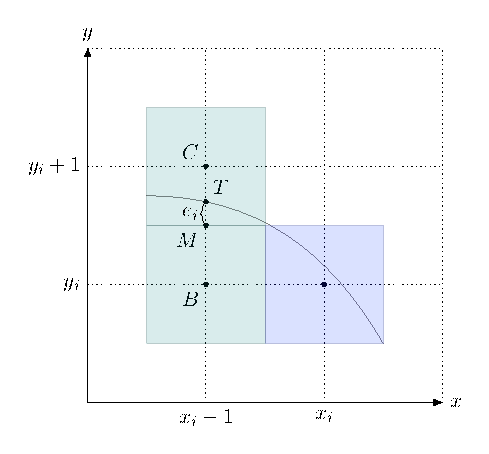
\includegraphics[scale=1]{Figures/Chapter1/Ellipse/figure3.pdf}
  \end{center}
  \caption{Περιοχή 2}
\end{figure}
Αντίστοιχη διαδικασία ισχύει και για την περιοχή 2. Συγκεκριμένα προκύπτει ότι:

\begin{table}[htb]
    \centering
    \begin{tabular}{@{}c|c@{}}
        \toprule
        $f_{mid2,i+1}$ & Επιλογή Σημείου \\
        \midrule
        $f_{mid2,i} - 2b^2 x_{i+1} + b^2$ & B \\
        $f_{mid2,i} - 2b^2 x_{i+1} + b^2 - 2a^2 x_{i+1}$ & D \\
        \bottomrule
    \end{tabular}
\end{table}

\subsection{Καθορισμός συνόρου μεταξύ της περιοχής 1 \& 2}

Επειδή η αλλαγή της περιοχής γίνεται στο σημείο όπου η κλίση της εφαπτομένης ισούται με -1 υπολογίζουμε την παράγωγο της εξίσωσης της έλλειψης:

\begin{equation}
    y^2 = b^2 - \frac{b^2}{a^2} x^2, \quad \frac{dy}{dx} = - \frac{2b^2 x}{2a^2 y}
\end{equation}

\begin{equation}
    \frac{dy}{dx} > -1 \Rightarrow 2a^2 y > 2b^2 x
\end{equation}

Όταν λοιπόν $2a^2 y > 2b^2 x$ έχουμε περάσει από την περιοχή 1 στην περιοχή 2. Για την ανάπτυξη του αλγορίθμου της έλλειψης θα ήταν επιθυμητό να χρησιμοποιήσουμε μόνο μια μεταβλητή απόφασης. Παρατηρούμε ότι η μετάβαση από το σύνορο μπορεί να υπολογισθεί με βάση την $f_{mid1}$. Συγκεκριμένα παρατηρούμε ότι:

\begin{equation}
    f_{mid2} - f_{mid1} = \left( b^2 x_i + a^2 y_i \right) + \frac{3}{4} \left( b^2 - a^2 \right)
\end{equation}

Τελικά

\begin{equation}
    f_{mid2} = f_{mid1} - \frac{2b^2 x_i + 2a^2 y_i}{2} + 0.75 \left( b^2 - a^2 \right)
\end{equation}

\begin{lstlisting}[caption={Γενικός αλγόριθμος σχερδιασμού ελλειψής του Bresenham }]
function elipsis(a, b, color)
    hold on
    x = a;
    y = 0;
    asqr = a^2;
    bsqr = b^2;
    a22 = 2 * asqr;
    b22 = 2 * bsqr;
    xslope = b22 * a;
    yslope = 0;
    fmid = bsqr * (0.25 - x) + asqr;

    % Area 1
    while (xslope > yslope)
        image(x, y, color)
        image(-x, -y, color)
        image(x, -y, color)
        image(-x, y, color)
        y = y + 1;
        yslope = yslope + a22;

        if fmid >= 0
            x = x - 1;
            xslope = xslope - b22;
            fmid = fmid - xslope;
        end
        fmid = fmid + yslope + asqr;
    end

    % Border correction
    fmid = fmid - (yslope + xslope)/2 + 0.75 * (bsqr - asqr);

    % Area 2
    while (x > 0)
        image(x, y, color)
        image(-x, -y, color)
        image(x, -y, color)
        image(-x, y, color)
        x = x - 1;
        xslope = xslope - b22;

        if fmid <= 0
            y = y + 1;
            yslope = yslope + a22;
            fmid = fmid + yslope;
        end
        fmid = fmid - xslope + bsqr;
    end
endfunction
\end{lstlisting}

	
\newpage	
	
\section*{Ασκήσεις 1ου Κεφαλαίου}

\begin{exercise}

Να κατασκευαστεί ο αλγόριθμος Plotline για την περίπτωση που η κλίση είναι μεγαλύτερη της μονάδας ($s>1$).
\end{exercise}

\begin{solution}
	
Στην περίπτωση που ισχύει $s >1$ είναι προτιμότερο η εξίσωση της ευθείας να επιλυθεί ως προς $x$, δηλαδή να εξαχθεί μία σχέση της μορφής $x = f (y)$. Τότε, ο αλγόριθμος \texttt{Plotline} λαμβάνει την ακόλουθη μορφή:
	
	
\begin{lstlisting} 
x1, y1 = get_coordinates("Give the coordinates of P1 e.g. (1,2):")
x2, y2 = get_coordinates("Give the coordinates of P2:")
s = (x2-x1) / (y2-y1)
c = (x_1y_2-x2y1 ) / (y2-y1)
for y = y1:y2
	x = round(sy+c) 
	plot(x,y)
end
\end{lstlisting}

Στον παραπάνω αλγόριθμο έχει θεωρηθεί ως δεδομένο ότι $s > 1$. Θα μπορούσε να κατασκευαστεί αλγόριθμος που να ενσωματώνει τις δύο περιπτώσεις, ελέγχοντας στην αρχή την τιμή κλίσης s (\texttt{if s < 1...else...}).


\end{solution}

\begin{exercise}

Να κατασκευαστεί ο αλγόριθμος του Bresenham για ευθεία, για το δεύτερο οκταμόριο.
\end{exercise}

\begin{solution}
	Στο δεύτερο οκταμόριο ισχύει $s >1$, οπότε είναι προτιμότερο η εξίσωση της ευθείας να επιλυθεί ως προς $x$, δηλαδή να εξαχθεί μία σχέση της μορφής $x= f (y)$. Τότε, ο αλγόριθμος του Bresenham λαμβάνει την ακόλουθη μορφή:
	
\begin{lstlisting}[caption={Bresenham Algorithm for 2nd Octant Line Algorithm}]
	x1, y1 = get_coordinates("Give the coordinates of P1 e.g. (1,2):")
	x2, y2 = get_coordinates("Give the coordinates of P2:")
	Dx = x2 - x1
	Dy = y2-y1
	x = x1
	y = y1
	c1 = 2Dx
	error = c1 - Dy
	c2 = error - Dy
	while y <= y2
		if error <0
			error = error + c1
		else
			x = x+1
			error = error + c2
		plot(x,y)
		y = y + 1
		end
	end	
\end{lstlisting}


\end{solution}
\begin{exercise}

Να κατασκευαστεί ο αλγόριθμος του Bresenham για ευθεία, για το δεύτερο οκταμόριο.
\end{exercise}

\begin{solution}
	Στο δεύτερο οκταμόριο ισχύει $s >1$, οπότε είναι προτιμότερο η εξίσωση της ευθείας να επιλυθεί ως προς $x$, δηλαδή να εξαχθεί μία σχέση της μορφής $x= f (y)$. Τότε, ο αλγόριθμος του Bresenham λαμβάνει την ακόλουθη μορφή:
	
\begin{lstlisting}[caption={Bresenham Algorithm for 2nd Octant Line Algorithm}]
	x1, y1 = get_coordinates("Give the coordinates of P1 e.g. (1,2):")
	x2, y2 = get_coordinates("Give the coordinates of P2:")
	Dx = x2 - x1
	Dy = y2-y1
	x = x1
	y = y1
	c1 = 2Dx
	error = c1 - Dy
	c2 = error - Dy
	while y <= y2
		if error <0
			error = error + c1
		else
			x = x+1
			error = error + c2
		plot(x,y)
		y = y + 1
		end
	end	
\end{lstlisting}


\end{solution}
\begin{exercise}
		 Να κατασκευαστεί ο αλγόριθμος του Bresenham για το σχεδιασμό κύκλου κέντρου $O(0,0)$ και ακτίνας $r$, στο πρώτο οκταμόριο.
\end{exercise}

\begin{solution}


Η μετατροπή του βασικού αλγορίθμου του Bresenham αφορά τη συμμετρία ως προς την ευθεία $y = x$. Συγκεκριμένα, η μετατροπή αφορά την εκτύπωση του σημείου $(y, x)$ αντί του σημείου $(x, y)$ στην εντολή \texttt{plot}:

\begin{lstlisting} 
r = readline()
x = 0
y = r
error = 3 - 2r
while x <= y
    plot(y, x)
    x = x + 1
    if error ≥ 0
        y = y - 1
        error = error - 4y
    end
    error = error + 4x + 2
end

\end{lstlisting}

\end{solution}
\begin{exercise}
		 Να κατασκευαστεί ο αλγόριθμος του Bresenham για το σχεδιασμό κύκλου κέντρου $O(0,0)$ και ακτίνας $r$, στο πρώτο οκταμόριο.
\end{exercise}

\begin{solution}


Η μετατροπή του βασικού αλγορίθμου του Bresenham αφορά τη συμμετρία ως προς την ευθεία $y = x$. Συγκεκριμένα, η μετατροπή αφορά την εκτύπωση του σημείου $(y, x)$ αντί του σημείου $(x, y)$ στην εντολή \texttt{plot}:

\begin{lstlisting} 
r = readline()
x = 0
y = r
error = 3 - 2r
while x <= y
    plot(y, x)
    x = x + 1
    if error ≥ 0
        y = y - 1
        error = error - 4y
    end
    error = error + 4x + 2
end

\end{lstlisting}

\end{solution}
\begin{exercise}
	Δίνονται τα σημεία $P_1 (3,5), P_2(7,7), P_3 (8,6)$. Θεωρώντας ότι το pixel που αντιστοιχεί στο $P_1(3,5)$ φωτίζεται στην οθόνη, να προσδιοριστούν στην οθόνη για τον σχεδιασμό των ευθυγράμμων τμημάτων $P_1 P_2, P_1 P_3$.

\begin{enumerate}
  \item[i)] Θεωρώντας ότι το pixel που αντιστοιχεί στο $P_1 (3,5) $ φωτίζεται στην οθόνη, να προσδιορισθούν οι συντεταγμένες των επόμενων pixels που θα φωτισθούν στην οθόνη για το σχεδιασμό των ευθυγράμμων τμημάτων $P_1 P_2, P_1 P _3$.
  \item[ii)]   Επιπλέον να μελετήσετε τον σχεδιασμό των ευθυγράμμων τμημάτων: \newline 
	$P_4 P_5, P_6 P_7, P_8 P_9, P_{10} P_{11}$.
\end{enumerate}

\begin{figure}[hbt]
  \begin{center}
	\includegraphics[scale=0.7]{Chapter1/Exercises/ex13/graph1.pdf}
  \end{center}
  \caption{Παράσταση ζητούμενων ευθυγράμμων τμημάτων}
\end{figure}


		
\end{exercise}

\begin{solution}

\begin{enumerate}
	
\item[i)] Γενικά ο αλγόριθμος του Bresenham για ευθείες στο πρώτο οκταμόριο είναι:

\begin{lstlisting}[caption={Αλγόριθμος του Bresenham για ζητούμενο ευθύγραμμο τμήμα}]
x1, y1 = get_coordinates("Give the coordinates of P1 e.g. (1,2):")
x2, y2 = get_coordinates("Give the coordinates of P2:")
Dx = x2 - x1
Dy = y2-y1
x = x1
y = y1
c1 = 2Dy
er = c1 - Dx
c2 = er - Dx
while x <= 7
    plot(x,y)
    x = x+1
    if er <0
        er = er + c1
    else
        y = y+1
        er = er + c2
    plot(x,y)
    end
end	
\end{lstlisting}

Για τα σημεία $P_1(3,5)$ και $P_2(7,7)$ θα έχουμε:

\begin{itemize}[noitemsep, topsep=0pt] % Reduce vertical spacing
\begin{multicols}{2} % Split into 2 columns
  \item $x = x_1 = 3$
  \item $y = y_1 = 5$
  \item $\Delta x = x_2 - x_1 = 5 - 3 = 4$
  \item $\Delta y = y_2 - y_1 = 7 - 5 = 2$
  \item $c_1 = 2 \cdot \Delta y = 2 \cdot 2 = 4$
  \item $er = c_1 - \Delta x = 4 - 4 = 0$
  \item $c_2 = er - \Delta x = 0 - 4 = -4$
\end{multicols}
\end{itemize}

Ο αλγόριθμος θα τρέξει ως εξής:

\lstset{style=tt} 
    
\begin{itemize}
  \item \underline{1η επανάληψη}

		\begin{lstlisting}
		x == 3 $<=$ 7 $\Rightarrow$
			plot(3,5) 
			x  = 4 %(x == x+1) 
			er == 0 $\geq$ 0 
				y = 6 %(y == y+1 == 6) 
				er = -4 %(er == er + c2 == 0 +(-4) == -4)
		\end{lstlisting}
		
	\item  \underline{2η επανάληψη}
		
		\begin{lstlisting}
		x == 4 $\leq$ 7 $\Rightarrow$
			plot(4,6)
			x = 5 %(x == x+1 == 5)
			er == -4 $<$ 0 $\Rightarrow$
				er = 0 %(er == er + c1 == -4 + 4 == 0)
		\end{lstlisting}		
				
	\item	\underline{3η επανάληψη}
		\begin{lstlisting}
		x == 5 $\leq$ 7 $\Rightarrow$
			plot(5,6)
			x = 6 %(x == x+1 == 6)
			er == 0 $\geq$ 0 $\Rightarrow$
				y = 7 %(y == y+1 == 7)
				er = -4 %(er == er + c2 == 0 +(-4) == -4)	
		\end{lstlisting}		
		
	\item	\underline{4η επανάληψη}
		\begin{lstlisting}
		x == 6 $\leq$ 7 $\Rightarrow$
			plot(6,7)
			x = 7 %(x == x+1 == 7)
			er == -4 $<$ 0 $\Rightarrow$
				er = 4 %(er == er + c1 == -4 + 4 == 0)		
		\end{lstlisting}
				
	\item	\underline{5η επανάληψη}
		\begin{lstlisting}
		x == 7 $\leq$ 7 $\Rightarrow$
			plot(7,7)
			x = 8 %(x == x+1 == 8)
			er == 4 $\geq$ 0 $\Rightarrow$
				y = 8 %(y == y+1 == 8)
				er = 8 %(er == er + c1 == 4 + 4 == 8)
		\end{lstlisting}
		
	\item	\underline{6η επανάληψη}
		\begin{lstlisting}
		x == 8 $>$ 7 $\Rightarrow$ %STOP
		\end{lstlisting}
\end{itemize}					


Συνολικά θα φωτιστούν τα σημεία : $(4, 6), (5, 6), (6, 7), (7,7)$.

Για τα σημεία $P_1(3,5)$ και $P_2(8,6)$ έχουμε:


\begin{itemize}[noitemsep, topsep=0pt] % Reduce vertical spacing
\begin{multicols}{2} % Split into 2 columns
  \item $x = x_1 = 3$
  \item $y = y_1 = 5$
  \item $\Delta x = x_2 - x_1 = 8 - 3 = 5$
  \item $\Delta y = y_2 - y_1 = 6 - 5 = 1$
  \item $c_1 = 2 \cdot \Delta y = 2 \cdot 1 = 2$
  \item $er = c_1 - \Delta x = 2 - 5 = -3$
  \item $c_2 = er - \Delta x = -3 - 5 = -8$
\end{multicols}
\end{itemize}


\begin{itemize}
\item \underline{1η επανάληψη}

\begin{lstlisting}
%Iteration 1:
x = 3 $\leq$ 8 $\Rightarrow$
    plot(3,5)
    x = 4 %(x = x+1 = 4)
    er = -3 < 0 $\Rightarrow$
        er = -1 %(er = er + c1 = -3 + 2 = -1)
    plot(4,5)
\end{lstlisting}

\item \underline{2η επανάληψη}

		\begin{lstlisting}
%Iteration 2:
x = 4 $\leq$ 8 $\Rightarrow$
    plot(4,5)
    x = 5 %(x = x+1 = 5)
    er = -1 < 0 $\Rightarrow$
        er = 1 %(er = er + c1 = -1 + 2 = 1)
    plot(5,5)
\end{lstlisting}

\item \underline{3η επανάληψη}

		\begin{lstlisting}
%Iteration 3:
x = 5 $\leq$ 8 $\Rightarrow$
    plot(5,5)
    x = 6 %(x = x+1 = 6)
    er = 1 >= 0 $\Rightarrow$
        y = 6 %(y = y+1 = 6)
        er = -7 %(er = er + c2 = 1 + (-8) = -7)
    plot(6,6)
\end{lstlisting}

\item \underline{4η επανάληψη}

		\begin{lstlisting}
%Iteration 4:
x = 6 $\leq$ 8 $\Rightarrow$
    plot(6,6)
    x = 7 %(x = x+1 = 7)
    er = -7 < 0 $\Rightarrow$
        er = -5 %(er = er + c1 = -7 + 2 = -5)
    plot(7,6)
\end{lstlisting}

\item \underline{5η επανάληψη}

		\begin{lstlisting}
%Iteration 5:
x = 7 $\leq$ 8 $\Rightarrow$
    plot(7,6)
    x = 8 %(x = x+1 = 8)
    er = -5 < 0 $\Rightarrow$
        er = -3 %(er = er + c1 = -5 + 2 = -3)
    plot(8,6)
\end{lstlisting}

\item \underline{6η επανάληψη}
\begin{lstlisting}
%Iteration 6:
x = 8 $\leq$ 8 $\Rightarrow$
    plot(8,6)
    x = 9 %(x = x+1 = 9)
    er = -3 < 0 $\Rightarrow$
        er = -1 %(er = er + c1 = -3 + 2 = -1)
    plot(9,6)
\end{lstlisting}

\end{itemize}

Συνολικά θα φωτιστούν τα σημεία : $(4, 5), (5, 5), (6, 6), (7,6), (8,6)$.	

\end{enumerate}
	
\end{solution}
\begin{exercise}
	Δίνονται τα σημεία $P_1(3, 5), P_2 (9, 18)$ Θεωρώντας ότι το σημείο $P_1$ φωτίζεται στην οθόνη, εφαρμόστε τον αλγόριθμο του Bresenham για τον υπολογισμό των $5$ αμέσως επόμενων pixels που θα φωτισθούν κατα τη σχεδίαση του ευθύγραμμου τμήματος $P_1 P_2$.	
\end{exercise}


\begin{solution}

Όπως έχουμε δει στη θεωρία, προκειμένου να σχεδιάσουμε την ευθεία του Bresenham για σημεία που ανήκουν στο 2ο οκταμόριο, μπορούμε να χρησιμοποιήσουμε τα συμμετρικά των σημείων $P_1, P_2$ ως προς την $1$η διχοτόμο, τα οποία θα ανήκουν στο 1ο οκταμόριο. Άρα θα χρησιμοποιήσουμε τα σημεία $P_1^{'}(5,3)$ και $P_2^{'}(18,9)$ και θα χρησιμοποιήσουμε τον γνωστό αλγόριθμο του Bresenham για σχεδιασμό ευθυγράμμου τμήματος στο 1ο οκταμόριο ως εξής:

\begin{lstlisting}[caption={Αλγόριθμος του Bresenham για 1ο οκταμόριο}]
x1, y1 = get_coordinates("Give the coordinates of P1 e.g. (1,2):")
x2, y2 = get_coordinates("Give the coordinates of P2:")
Dx = x2 - x1
Dy = y2 - y1
x = x1
y = y1
c1 = 2 * Dy
er = c1 - Dx
c2 = er - Dx
while x <= 18
    plot(x, y)
    x = x + 1
    if er < 0
        er = er + c1
    else
        y = y + 1
        er = er + c2
    plot(x, y)
end
\end{lstlisting}


Για τα σημεία \( P_1^{'}(5, 3) \) και \( P_2^{'}(18, 9) \) θα έχουμε:

\begin{itemize}[noitemsep, topsep=0pt] % Reduce vertical spacing
\begin{multicols}{2} % Split into 2 columns
  \item \( x = x_1 = 5 \)
  \item \( y = y_1 = 3 \)
  \item \( \Delta x = x_2 - x_1 = 18 - 5 = 13 \)
  \item \( \Delta y = y_2 - y_1 = 9 - 3 = 6 \)
  \item \( c_1 = 2 \cdot \Delta y = 2 \cdot 6 = 12 \)
  \item \( er = c_1 - \Delta x = 12 - 13 = -1 \)
  \item \( c_2 = er - \Delta x = -1 - 13 = -14 \)
\end{multicols}
\end{itemize}

Ο αλγόριθμος θα τρέξει ως εξής:

\lstset{style=tt} 

\begin{itemize}
  \item \underline{1η επανάληψη}

		\begin{lstlisting}
		x == 5 $<=$ 18 $\Rightarrow$
			plot(5, 3) 
			x = 6 %(x == x + 1) 
			er == -1 $<$ 0 
				er = 11 %(er == er + c1 == -1 + 12 == 11)
		\end{lstlisting}
		
	\item \underline{2η επανάληψη}
		
		\begin{lstlisting}
		x == 6 $\leq$ 18 $\Rightarrow$
			plot(6, 3)
			x = 7 %(x == x + 1 == 7)
			er == 11 $\geq$ 0 
				y = 4 %(y == y + 1 == 4)
				er = -3 %(er == er + c2 == 11 + (-14) == -3)
		\end{lstlisting}		
				
	\item \underline{3η επανάληψη}
		\begin{lstlisting}
		x == 7 $\leq$ 18 $\Rightarrow$
			plot(7, 4)
			x = 8 %(x == x + 1 == 8)
			er == -3 $<$ 0 
				er = 9 %(er == er + c1 == -3 + 12 == 9)
		\end{lstlisting}		
		
	\item \underline{4η επανάληψη}
		\begin{lstlisting}
		x == 8 $\leq$ 18 $\Rightarrow$
			plot(8, 4)
			x = 9 %(x == x + 1 == 9)
			er == 9 $\geq$ 0 
				y = 5 %(y == y + 1 == 5)
				er = -5 %(er == er + c2 == 9 + (-14) == -5)
		\end{lstlisting}
				
	\item \underline{5η επανάληψη}
		\begin{lstlisting}
		x == 9 $\leq$ 18 $\Rightarrow$
			plot(9, 5)
			x = 10 %(x == x + 1 == 10)
			er == -5 $<$ 0 
				er = 7 %(er == er + c1 == -5 + 12 == 7)
		\end{lstlisting}
		
	\item \underline{6η επανάληψη}
		\begin{lstlisting}
		x == 10 $\leq$ 18 $\Rightarrow$
			plot(10, 5)
			x = 11 %(x == x + 1 == 11)
			er == 7 $\geq$ 0 
				y = 6 %(y == y + 1 == 6)
				er = -7 %(er == er + c2 == 7 + (-14) == -7)
		\end{lstlisting}
\end{itemize}

Τα $6$ πρώτα σημεία που θα φωτιστούν δηλαδή από τον αλγόριθμο με είσοδο τις συντεταγμένες $P_1^{'}$ και $P_2^{'}$, είναι: \( (5,3) \to (6, 3) \to (7, 4) \to (8, 4) \to (9, 5) \to (10, 5) \).

Για να βρούμε λοιπόν τα $5$ αμέσως επόμενων pixels που θα φωτισθούν κατα τη σχεδίαση του ευθύγραμμου τμήματος $P_1 P_2$ αρκεί να βρούμε τα συμμετρικά των παραπάνω φωτισμένων pixel ως προς την $1$η διχοτόμο.

Τα ζητούμενα δηλαδή σημεία, δεδομένου ότι θα φωτιστεί το pixel με κέντρο $(3,5)$ θα είναι: \newline 
$(3, 6) \to (4, 7) \to (4, 8) \to (5, 9) \to (5, 10) $

\begin{figure}[hbt]
  \begin{center}
	\includegraphics[scale=0.7]{Chapter1/Exercises/ex14/graph1.pdf}
  \end{center}
  \caption{Παράσταση ευθυγράμμων τμημάτων $P_1 P_2$ και $P_1^{'} P_2^{'}$ σύμφωνα με τον αλγόριθμο του Bresenham $P_1(3, 5), P_2 (9, 18)$ για σημεία $P_1^{'}(5, 3), P_2^{'} (18, 9)$}
\end{figure}


\end{solution}
\begin{exercise}

Να προσδιοριστούν οι πίνακες στροφής στο χώρο ενός αντικειμένου κατά γωνία $\theta$, ως προς τους άξονες $y'y$, $x'x$, $R_{\theta,y}$ και $R_{\theta,x}$ αντίστοιχα.	
\end{exercise}
\begin{solution}
	



\begin{itemize}
  \item  Για τη στροφή ως προς τον άξονα $y'y$ ισχύουν οι εξής μετασχηματισμοί:
\[
\begin{aligned}
    x' &= x\cos\theta + z\sin\theta, \\
    y' &= y, \\
    z' &= -x\sin\theta + z\cos\theta.
\end{aligned}
\]
Ο αντίστοιχος πίνακας είναι:
\[
R_{\theta,y} = \begin{bmatrix}
\cos\theta & 0 & \sin\theta & 0\\
0 & 1 & 0  & 0\\
-\sin\theta & 0 & \cos\theta & 0\\
0 & 0 & 0 & 1
\end{bmatrix}.
\]

\item Για τη στροφή ως προς τον άξονα $x'x$ ισχύουν οι εξής μετασχηματισμοί:

\[
\begin{aligned}
    x' &= x, \\
    y' &= y\cos\theta - z\sin\theta, \\
    z' &= y\sin\theta + z\cos\theta.
\end{aligned}
\]

Ο αντίστοιχος πίνακας είναι:
\[
R_{\theta,x} = \begin{bmatrix}
1 & 0 & 0 & 0\\
0 & \cos\theta & -\sin\theta & 0\\
0 & \sin\theta & \cos\theta & 0\\
0 & 0 & 0 & 1
\end{bmatrix}.
\]

\end{itemize}
\end{solution}
\begin{exercise}
	
Να υπολογιστούν ποια θα είναι τα τρία επόμενα προς φωτισμό pixels, σύμφωνα με τον αλγόριθμο του Bresenham, για σχεδιασμό κύκλου κέντρου $K(7,3)$ και ακτίνας $r = 5$, στο πρώτο οκταμόριο.
\end{exercise}
\begin{solution}
	

Το πρώτο σημείο είναι το $A(7+5, 3) \equiv A(12, 3)$. Για τα επόμενα σημεία, υπολογίζεται το κάθε σημείο σύμφωνα με τον αλγόριθμο του Bresenham με κέντρο το $O(0,0)$, στη συνέχεια το συμμετρικό του ως προς την ευθεία $y=x$ και τέλος μετατοπίζεται κατά $(7,3)$:


\underline{1η Επανάληψη}
\begin{itemize}
  \item $d_1 = y_1^2 - y^2 = y_1^2 - \left[ r^2 - (x_1 + 1)^2 \right] = 5^2 - \left[ 5^2 - (0+1)^2 \right] = 1,$
  \item $d_2 = y^2 - (y_1+1)^2 = \left[ r^2 - (x_1+1)^2 \right] - (y_1+1)^2 = \left[ 5^2 - (0+1)^2 \right] - (5+1)^2 = -12.$
\end{itemize}

Άρα $d_1 - d_2 = 1 - (-12) = 13 \geq 0 \\Rightarrow (1,4) \xRightarrow{\sim y = x} (4,1) \xRightarrow{+(7,3)} (11,4)$.


\underline{2η Επανάληψη}
\begin{itemize}
  \item $d_1 = y_2^2 - y^2 = y_2^2 - \left[ r^2 - (x_2 + 1)^2 \right] = 4^2 - \left[ 5^2 - (1+1)^2 \right] = -5,$
  \item $d_2 = y^2 - (y_2+1)^2 = \left[ r^2 - (x_2+1)^2 \right] - (y_2+1)^2 = \left[ 5^2 - (1+1)^2 \right] - (4+1)^2 = -4.$
\end{itemize}

Άρα $d_1 - d_2 = -5 - (-4) = -1 < 0 \\Rightarrow (2,4) \xRightarrow{\sim y = x} (4,2) \xRightarrow{+(7,3)} (11,5).$

\underline{3η Επανάληψη}
\begin{itemize}
  \item $d_1 = y_3^2 - y^2 = y_3^2 - \left[ r^2 - (x_3 + 1)^2 \right] = 4^2 - \left[ 5^2 - (2+1)^2 \right] = 0,$
  \item $d_2 = y^2 - (y_3+1)^2 = \left[ r^2 - (x_3+1)^2 \right] - (y_3+1)^2 = \left[ 5^2 - (2+1)^2 \right] - (4+1)^2 = -9.$
\end{itemize}

Άρα $d_1 - d_2 = 0 - (-9) = 9 \geq 0 \Rightarrow (3,3)  \xRightarrow{\sim y = x}(3,3) \xRightarrow{(+7,3)} (10,6).$




Δηλαδή τα pixels που θα φωτιστούν είναι τα: \newline $A(12,3) \to (11,4) \to (11,5) to (10,6)$.
\end{solution}
\begin{exercise}
	Να υπολογιστούν ποια θα είναι τα επόμενα προς φωτισμό pixels, σύμφωνα με τον αλγόριθμο του Bresenham, για σχεδιασμό κύκλου: 
\begin{enumerate}
  \item[i)] Στο 2ο οκταμόριο με  κέντρο $K(0,0)$ και ακτίνα $r=5$.
  \item[ii)] Στο 3ο οκταμόριο με  κέντρο $K(7,3)$ και ακτίνα $r=5$.
\end{enumerate}
		
\end{exercise}

\begin{exercise}
	Δίνεται κύκλος με κέντρο $Κ(7,7)$ και ακτίνα $r = 10$. 
	\begin{itemize}
	  \item Ποιό είναι το πρώτο pixel που θα φωτίσει ο αλγόριθμός σχεδιασμού κύκλου του Bresenham για το $2$ο οκταμόριο;
	  \item Ποια είναι τα $2$ αμέσως επόμενα pixel που θα φωτίσει ο αλγόριθμός σχεδιασμού κύκλου του Bresenham για το $2$ο οκταμόριο;
	  \item Να υπολογίστε  τα pixels που θα φωτισθούν από την εφαρμογή της συμμετρίας των $8$ δρόμων.
	\end{itemize}
\end{exercise}


\begin{solution}
	

\begin{lstlisting}[caption={Αλγόριθμος του Bresenham για σχεδιασμό κύκλου}]
function brescircle(xc, yc, r)
    # (xc, yc) are the coordinates of the circle's centre
    # r is the radius of the circle
    x = 0 
    y = r
    error = 3 - 2 * r
    
    while x <= y
        plot(x+xc, y+yc, 0)
        plot(x+xc, -y+yc, 0) 
        plot(-x+xc, y+yc, 0) 
        plot(-x+xc, -y+yc, 0) 
        plot(y+xc, x+yc, 0) 
        plot(-y+xc, x+yc, 0)
        plot(y+xc, -x+yc, 0) 
        plot(-y+xc, -x+yc, 0) 
        x = x + 1
        if error > 0
            y = y - 1
            error = error - 4*y
        end
        error = error + 4*x + 2
    end
end
\end{lstlisting}


Για τον κύκλο με κέντρο \( K(7, 7) \) και ακτίνα \( r = 10 \), θα έχουμε:

\begin{itemize}[noitemsep, topsep=0pt] % Reduce vertical spacing
\begin{multicols}{2} % Split into 2 columns
  \item \( x = 0 \)
  \item \( y = 10 \)
  \item \( error = 3 - 2 \cdot r = 3 - 20 = -17 \)
\end{multicols}
\end{itemize}


\begin{itemize}
  \item \underline{1η επανάληψη}
\lstset{style=tt}
		\begin{lstlisting}
		x == 0 $<=$ 10 $\Rightarrow$
			plot(7, 17) % (x+xc, y+yc)
			plot(7, -3)  % (x+xc, -y+yc)
			plot(-7, 17) % (-x+xc, y+yc)
			plot(-7, -3) % (-x+xc, -y+yc)
			plot(17, 7)  % (y+xc, x+yc)
			plot(-17, 7) % (-y+xc, x+yc)
			plot(17, -7) % (y+xc, -x+yc)
			plot(-17, -7) % (-y+xc, -x+yc)
			x = 1 %(x == x + 1)
			error == -17 $<$ 0 
				error = -17 + 4*1 + 2 = -11 %(error == error + 4*x + 2)
		\end{lstlisting}

  \item \underline{2η επανάληψη}

		\begin{lstlisting}
		x == 1 $<=$ 10 $\Rightarrow$
			plot(8, 17) % (x+xc, y+yc)
			plot(8, -3)  % (x+xc, -y+yc)
			plot(-8, 17) % (-x+xc, y+yc)
			plot(-8, -3) % (-x+xc, -y+yc)
			plot(17, 8)  % (y+xc, x+yc)
			plot(-17, 8) % (-y+xc, x+yc)
			plot(17, -8) % (y+xc, -x+yc)
			plot(-17, -8) % (-y+xc, -x+yc)
			x = 2 %(x == x + 1)
			error == -11 $<$ 0 
				error = -11 + 4*2 + 2 = -1 %(error == error + 4*x + 2)
		\end{lstlisting}

  \item \underline{3η επανάληψη}

		\begin{lstlisting}
		x == 2 $<=$ 10 $\Rightarrow$
			plot(9, 17) % (x+xc, y+yc)
			plot(9, -3)  % (x+xc, -y+yc)
			plot(-9, 17) % (-x+xc, y+yc)
			plot(-9, -3) % (-x+xc, -y+yc)
			plot(17, 9)  % (y+xc, x+yc)
			plot(-17, 9) % (-y+xc, x+yc)
			plot(17, -9) % (y+xc, -x+yc)
			plot(-17, -9) % (-y+xc, -x+yc)
			x = 3 %(x == x + 1)
			error == -1 $<$ 0 
				error = -1 + 4*3 + 2 = 13 %(error == error + 4*x + 2)
		\end{lstlisting}
\end{itemize}

\begin{figure}[hbt]
  \begin{center}
	\includegraphics[scale=0.6]{Chapter1/Exercises/ex15/graph1.pdf}
  \end{center}
  \caption{Παράσταση πρώτων $3$ επαναλήψεων αλγορίθμου Bresenham για κύκλο κέντρου $Κ(7,7)$ και ακτίνας $r = 10$. Τα χρώματα για την $1$η, $2$η και $3$η επανάληψη είναι μπλε και πορτοκαλί αντίστοιχα. }
\end{figure}

\end{solution}
\begin{exercise}
	Να κατασκευαστεί ο αλγόριθμος του Bresenham για το σχεδιασμό κύκλου κέντρου $Κ(x, y)$ και ακτίνας $r$, στο δεύτερο οκταμόριο.
\end{exercise}

\begin{solution}
	Η μετατροπή του βασικού αλγορίθμου του Bresenham αφορά τη μετακίνηση του κέντρου του κύκλου από το $O(0,0)$ στο $Κ(x_c, y_c)$. Συγκεκριμένα, η μετατροπή αφορά την εκτύπωση του σημείου $(x + x_c,y +y_c)$ αντί του σημείου $(x,y)$ στην εντολή plot :

\begin{lstlisting} 
r = readline() 
xc = readline() 
yc = readline() 
x=0
y = r
error = 3 -2r
while x <= y plot(x+xc, y+ yc)
	plot(x+xc, y+yc)
	x=x+1
	if error >= 0
		y=y-1
		error = error - 4y
	end
	error = error + 4x + 2 + c2
end
\end{lstlisting}		

\end{solution}
\begin{exercise}
	Δίνονται τα σημεία $P_1 (3,5), P_2(7,7), P_3 (8,6)$. Θεωρώντας ότι το pixel που αντιστοιχεί στο $P_1(3,5)$ φωτίζεται στην οθόνη, να προσδιοριστούν στην οθόνη για τον σχεδιασμό των ευθυγράμμων τμημάτων $P_1 P_2, P_1 P_3$.

\begin{enumerate}
  \item[i)] Θεωρώντας ότι το pixel που αντιστοιχεί στο $P_1 (3,5) $ φωτίζεται στην οθόνη, να προσδιορισθούν οι συντεταγμένες των επόμενων pixels που θα φωτισθούν στην οθόνη για το σχεδιασμό των ευθυγράμμων τμημάτων $P_1 P_2, P_1 P _3$.
  \item[ii)]   Επιπλέον να μελετήσετε τον σχεδιασμό των ευθυγράμμων τμημάτων: \newline 
	$P_4 P_5, P_6 P_7, P_8 P_9, P_{10} P_{11}$.
\end{enumerate}

\begin{figure}[hbt]
  \begin{center}
	\includegraphics[scale=0.7]{Chapter1/Exercises/ex13/graph1.pdf}
  \end{center}
  \caption{Παράσταση ζητούμενων ευθυγράμμων τμημάτων}
\end{figure}


		
\end{exercise}

\begin{solution}

\begin{enumerate}
	
\item[i)] Γενικά ο αλγόριθμος του Bresenham για ευθείες στο πρώτο οκταμόριο είναι:

\begin{lstlisting}[caption={Αλγόριθμος του Bresenham για ζητούμενο ευθύγραμμο τμήμα}]
x1, y1 = get_coordinates("Give the coordinates of P1 e.g. (1,2):")
x2, y2 = get_coordinates("Give the coordinates of P2:")
Dx = x2 - x1
Dy = y2-y1
x = x1
y = y1
c1 = 2Dy
er = c1 - Dx
c2 = er - Dx
while x <= 7
    plot(x,y)
    x = x+1
    if er <0
        er = er + c1
    else
        y = y+1
        er = er + c2
    plot(x,y)
    end
end	
\end{lstlisting}

Για τα σημεία $P_1(3,5)$ και $P_2(7,7)$ θα έχουμε:

\begin{itemize}[noitemsep, topsep=0pt] % Reduce vertical spacing
\begin{multicols}{2} % Split into 2 columns
  \item $x = x_1 = 3$
  \item $y = y_1 = 5$
  \item $\Delta x = x_2 - x_1 = 5 - 3 = 4$
  \item $\Delta y = y_2 - y_1 = 7 - 5 = 2$
  \item $c_1 = 2 \cdot \Delta y = 2 \cdot 2 = 4$
  \item $er = c_1 - \Delta x = 4 - 4 = 0$
  \item $c_2 = er - \Delta x = 0 - 4 = -4$
\end{multicols}
\end{itemize}

Ο αλγόριθμος θα τρέξει ως εξής:

\lstset{style=tt} 
    
\begin{itemize}
  \item \underline{1η επανάληψη}

		\begin{lstlisting}
		x == 3 $<=$ 7 $\Rightarrow$
			plot(3,5) 
			x  = 4 %(x == x+1) 
			er == 0 $\geq$ 0 
				y = 6 %(y == y+1 == 6) 
				er = -4 %(er == er + c2 == 0 +(-4) == -4)
		\end{lstlisting}
		
	\item  \underline{2η επανάληψη}
		
		\begin{lstlisting}
		x == 4 $\leq$ 7 $\Rightarrow$
			plot(4,6)
			x = 5 %(x == x+1 == 5)
			er == -4 $<$ 0 $\Rightarrow$
				er = 0 %(er == er + c1 == -4 + 4 == 0)
		\end{lstlisting}		
				
	\item	\underline{3η επανάληψη}
		\begin{lstlisting}
		x == 5 $\leq$ 7 $\Rightarrow$
			plot(5,6)
			x = 6 %(x == x+1 == 6)
			er == 0 $\geq$ 0 $\Rightarrow$
				y = 7 %(y == y+1 == 7)
				er = -4 %(er == er + c2 == 0 +(-4) == -4)	
		\end{lstlisting}		
		
	\item	\underline{4η επανάληψη}
		\begin{lstlisting}
		x == 6 $\leq$ 7 $\Rightarrow$
			plot(6,7)
			x = 7 %(x == x+1 == 7)
			er == -4 $<$ 0 $\Rightarrow$
				er = 4 %(er == er + c1 == -4 + 4 == 0)		
		\end{lstlisting}
				
	\item	\underline{5η επανάληψη}
		\begin{lstlisting}
		x == 7 $\leq$ 7 $\Rightarrow$
			plot(7,7)
			x = 8 %(x == x+1 == 8)
			er == 4 $\geq$ 0 $\Rightarrow$
				y = 8 %(y == y+1 == 8)
				er = 8 %(er == er + c1 == 4 + 4 == 8)
		\end{lstlisting}
		
	\item	\underline{6η επανάληψη}
		\begin{lstlisting}
		x == 8 $>$ 7 $\Rightarrow$ %STOP
		\end{lstlisting}
\end{itemize}					


Συνολικά θα φωτιστούν τα σημεία : $(4, 6), (5, 6), (6, 7), (7,7)$.

Για τα σημεία $P_1(3,5)$ και $P_2(8,6)$ έχουμε:


\begin{itemize}[noitemsep, topsep=0pt] % Reduce vertical spacing
\begin{multicols}{2} % Split into 2 columns
  \item $x = x_1 = 3$
  \item $y = y_1 = 5$
  \item $\Delta x = x_2 - x_1 = 8 - 3 = 5$
  \item $\Delta y = y_2 - y_1 = 6 - 5 = 1$
  \item $c_1 = 2 \cdot \Delta y = 2 \cdot 1 = 2$
  \item $er = c_1 - \Delta x = 2 - 5 = -3$
  \item $c_2 = er - \Delta x = -3 - 5 = -8$
\end{multicols}
\end{itemize}


\begin{itemize}
\item \underline{1η επανάληψη}

\begin{lstlisting}
%Iteration 1:
x = 3 $\leq$ 8 $\Rightarrow$
    plot(3,5)
    x = 4 %(x = x+1 = 4)
    er = -3 < 0 $\Rightarrow$
        er = -1 %(er = er + c1 = -3 + 2 = -1)
    plot(4,5)
\end{lstlisting}

\item \underline{2η επανάληψη}

		\begin{lstlisting}
%Iteration 2:
x = 4 $\leq$ 8 $\Rightarrow$
    plot(4,5)
    x = 5 %(x = x+1 = 5)
    er = -1 < 0 $\Rightarrow$
        er = 1 %(er = er + c1 = -1 + 2 = 1)
    plot(5,5)
\end{lstlisting}

\item \underline{3η επανάληψη}

		\begin{lstlisting}
%Iteration 3:
x = 5 $\leq$ 8 $\Rightarrow$
    plot(5,5)
    x = 6 %(x = x+1 = 6)
    er = 1 >= 0 $\Rightarrow$
        y = 6 %(y = y+1 = 6)
        er = -7 %(er = er + c2 = 1 + (-8) = -7)
    plot(6,6)
\end{lstlisting}

\item \underline{4η επανάληψη}

		\begin{lstlisting}
%Iteration 4:
x = 6 $\leq$ 8 $\Rightarrow$
    plot(6,6)
    x = 7 %(x = x+1 = 7)
    er = -7 < 0 $\Rightarrow$
        er = -5 %(er = er + c1 = -7 + 2 = -5)
    plot(7,6)
\end{lstlisting}

\item \underline{5η επανάληψη}

		\begin{lstlisting}
%Iteration 5:
x = 7 $\leq$ 8 $\Rightarrow$
    plot(7,6)
    x = 8 %(x = x+1 = 8)
    er = -5 < 0 $\Rightarrow$
        er = -3 %(er = er + c1 = -5 + 2 = -3)
    plot(8,6)
\end{lstlisting}

\item \underline{6η επανάληψη}
\begin{lstlisting}
%Iteration 6:
x = 8 $\leq$ 8 $\Rightarrow$
    plot(8,6)
    x = 9 %(x = x+1 = 9)
    er = -3 < 0 $\Rightarrow$
        er = -1 %(er = er + c1 = -3 + 2 = -1)
    plot(9,6)
\end{lstlisting}

\end{itemize}

Συνολικά θα φωτιστούν τα σημεία : $(4, 5), (5, 5), (6, 6), (7,6), (8,6)$.	

\end{enumerate}
	
\end{solution}


